\documentclass{article}
% Packages used
% Packages
\usepackage{amssymb,amsmath,amsthm,bbm}
\usepackage{verbatim,float,url,dsfont}
\usepackage{graphicx,subfigure,psfrag}
\usepackage{algorithm,algorithmic}
\usepackage{mathtools,enumitem}
\usepackage{multirow}
\usepackage{ragged2e}
\usepackage{xr-hyper}
\usepackage{array}

\usepackage[colorlinks=true,citecolor=blue,urlcolor=blue,linkcolor=blue]{hyperref}
\usepackage[margin=1in]{geometry}
\usepackage[round]{natbib}

\usepackage[utf8]{inputenc} % allow utf-8 input
\usepackage[T1]{fontenc}    % use 8-bit T1 fonts
\usepackage{booktabs}       % professional-quality tables
\usepackage{nicefrac}         % compact symbols for 1/2, etc.
\usepackage{microtype}      % microtypography
\usepackage{pdflscape}

\ifdefined\TimesFont 
\usepackage{times} % use times font
\fi

\ifdefined\ParSkip 
\usepackage{parskip} % use par skip
\fi

% Place page number
\def\fillandplacepagenumber{%
 \par\pagestyle{empty}%
 \vbox to 0pt{\vss}\vfill
 \vbox to 0pt{\baselineskip0pt
   \hbox to\linewidth{\hss}%
   \baselineskip\footskip
   \hbox to\linewidth{%
     \hfil\thepage\hfil}\vss}}
     
% Theorems and such
\newtheorem{theorem}{Theorem}
\newtheorem{lemma}{Lemma}
\newtheorem{corollary}{Corollary}
\newtheorem{proposition}{Proposition}
\theoremstyle{definition}
\newtheorem{remark}{Remark}
\newtheorem{definition}{Definition}

% Assumption
\newtheorem*{assumption*}{\assumptionnumber}
\providecommand{\assumptionnumber}{}
\makeatletter
\newenvironment{assumption}[2]{
  \renewcommand{\assumptionnumber}{Assumption #1#2}
  \begin{assumption*}
  \protected@edef\@currentlabel{#1#2}}
{\end{assumption*}}
\makeatother

% Widebar
\makeatletter
\newcommand*\rel@kern[1]{\kern#1\dimexpr\macc@kerna}
\newcommand*\widebar[1]{%
  \begingroup
  \def\mathaccent##1##2{%
    \rel@kern{0.8}%
    \overline{\rel@kern{-0.8}\macc@nucleus\rel@kern{0.2}}%
    \rel@kern{-0.2}%
  }%
  \macc@depth\@ne
  \let\math@bgroup\@empty \let\math@egroup\macc@set@skewchar
  \mathsurround\z@ \frozen@everymath{\mathgroup\macc@group\relax}%
  \macc@set@skewchar\relax
  \let\mathaccentV\macc@nested@a
  \macc@nested@a\relax111{#1}%
  \endgroup
}
\makeatother

% Min and max 
\DeclareMathOperator*{\argmin}{argmin}
\DeclareMathOperator*{\argmax}{argmax}
\DeclareMathOperator*{\minimize}{minimize}
\DeclareMathOperator*{\maximize}{maximize}
\DeclareMathOperator*{\find}{find}
\DeclareMathOperator{\st}{subject\,\,to}

% Other operators
\DeclareMathOperator{\Cov}{Cov}
\DeclareMathOperator{\Var}{Var}
\DeclareMathOperator{\dm}{dim}
\DeclareMathOperator{\col}{col}
\DeclareMathOperator{\row}{row}
\DeclareMathOperator{\nul}{null}
\DeclareMathOperator{\rank}{rank}
\DeclareMathOperator{\nuli}{nullity}
\DeclareMathOperator{\spa}{span}
\DeclareMathOperator{\sign}{sign}
\DeclareMathOperator{\supp}{supp}
\DeclareMathOperator{\diag}{diag}
\DeclareMathOperator{\aff}{aff}
\DeclareMathOperator{\conv}{conv}
\DeclareMathOperator{\dom}{dom}
\DeclareMathOperator{\tr}{tr}
\DeclareMathOperator{\df}{df}

% Other shortcuts 
\def\R{\mathbb{R}}
\def\C{\mathbb{C}}
\def\E{\mathbb{E}}
\def\P{\mathbb{P}}
\def\T{\mathsf{T}}
\def\half{\frac{1}{2}}
\def\df{\mathrm{df}}
\def\hy{\hat{y}}
\def\hf{\hat{f}}
\def\hmu{\hat{\mu}}
\def\halpha{\hat{\alpha}}
\def\hbeta{\hat{\beta}}
\def\htheta{\hat{\theta}}
\def\indep{\perp\!\!\!\perp}
\def\th{^{\textnormal{th}}}

\def\cA{\mathcal{A}}
\def\cB{\mathcal{B}}
\def\cD{\mathcal{D}}
\def\cE{\mathcal{E}}
\def\cF{\mathcal{F}}
\def\cG{\mathcal{G}}
\def\cK{\mathcal{K}}
\def\cH{\mathcal{H}}
\def\cI{\mathcal{I}}
\def\cL{\mathcal{L}}
\def\cM{\mathcal{M}}
\def\cN{\mathcal{N}}
\def\cP{\mathcal{P}}
\def\cS{\mathcal{S}}
\def\cT{\mathcal{T}}
\def\cW{\mathcal{W}}
\def\cX{\mathcal{X}}
\def\cY{\mathcal{Y}}
\def\cZ{\mathcal{Z}}

 \def\given{\, \vert\, }

\def\TimesFont{} 
\graphicspath{{gfx/}}

\newcommand{\beginsupplement}{
  \setcounter{table}{0}  
  \renewcommand{\thetable}{S\arabic{table}} 
  \setcounter{figure}{0} 
  \renewcommand{\thefigure}{S\arabic{figure}}
  \setcounter{section}{0} 
  \renewcommand{\thesection}{S\arabic{section}}
}
\font\supptitlefont=cmr12 at 16pt 
\newcommand{\attn }[1]{\textcolor{red}{ATTN: #1}}
     
\begin{document}
\title{Retrospective estimation of latent COVID-19 infections before Omicron in the \US}
\author{Rachel Lobay, Maria Jahja, Ajitesh Srivastava, Ryan J.\ Tibshirani, Daniel J.\ McDonald}
\date{Version: \today}
\maketitle

\begin{abstract}
The true timing and magnitude of COVID-19 infections (rather than reported
cases) are of interest to both the public and to public health, but these are
challenging to pin down for a variety of data-driven and methodological reasons.
Accurate estimates of latent COVID-19 infections can improve our understanding
of the size and scope of the pandemic and provide more meaningful and timely
quantification of disease patterns and burden. In this work, we estimate daily
incident \emph{infections} for each \US state. Rather than taking a model-based
approach, our methods operate directly on data. We first deconvolve reported
COVID-19 cases to their infection date using delay distributions estimated from
the CDC linelist. We combine these deconvolved cases with serology data to scale
up to unreported infections. Our results cover all states at the daily
frequency, incorporate variant-specific incubation periods, and account for
reinfections and waning antigenic immunity. This analysis also produces
estimates for other important quantities such as the number of deconvolved cases
specific to each variant and the infection-case-report ratio. We also discuss some
implications of our results: a disease burden that appears earlier and more
extensively than previously quantified; differential infection-hospitalization
ratio estimates. Our findings help to better understand the impact of the
pandemic in the \US prior to the onset of Omicron and its descendants. 

\end{abstract}

\section{Introduction}

Reported COVID-19 cases are a staple in tracking the pandemic at varying
geographic resolutions \citep{dong2020interactive, nyt2020corona,
wp2020tracking}. Yet, for every case that is eventually reported to public
health, several infections are likely to have occurred, likely much earlier. To
see why, it is important to understand \emph{whose} cases are being reported and
what differentiates them from the unreported cases as well as \emph{when} these
case reports happen. \autoref{fig:chain_events_onset_report} shows an
illustration of the path of a symptomatic infection that \emph{is} eventually
reported to public health. Using this figure, we can discern a number of sources
of bias in the reporting pipeline. For instance, diagnostic testing mainly
targets symptomatic individuals; thus, infected individuals exhibiting little to
no symptoms are omitted \citep{cdc2022estimated}. In addition, testing
practices, availability, and uptake vary temporally and spatially
\citep{pitzer2021impact, ecdc2020strategies, hitchings2021usefulness}. Finally,
cases provide a belated view of the pandemic's progression, because they are
subject to delays due to the viral incubation period, the speed and severity of
symptom onset, laboratory confirmation, test turnaround times, and eventual
submission to public health \citep{pellis2021challenges, wash2020dash}. For
these reasons, reported cases are a lagging indicator of the course of the
pandemic. Furthermore, they do not represent the actual number of new infections
that occur on a given day as indicated by exposure to the pathogen. Since there
was no large-scale surveillance effort in the United States that reliably
tracked symptom onset, let alone infection onset, ascertaining the onset of all
\emph{infections} is challenging.

\begin{figure}[!tb]
\centering
    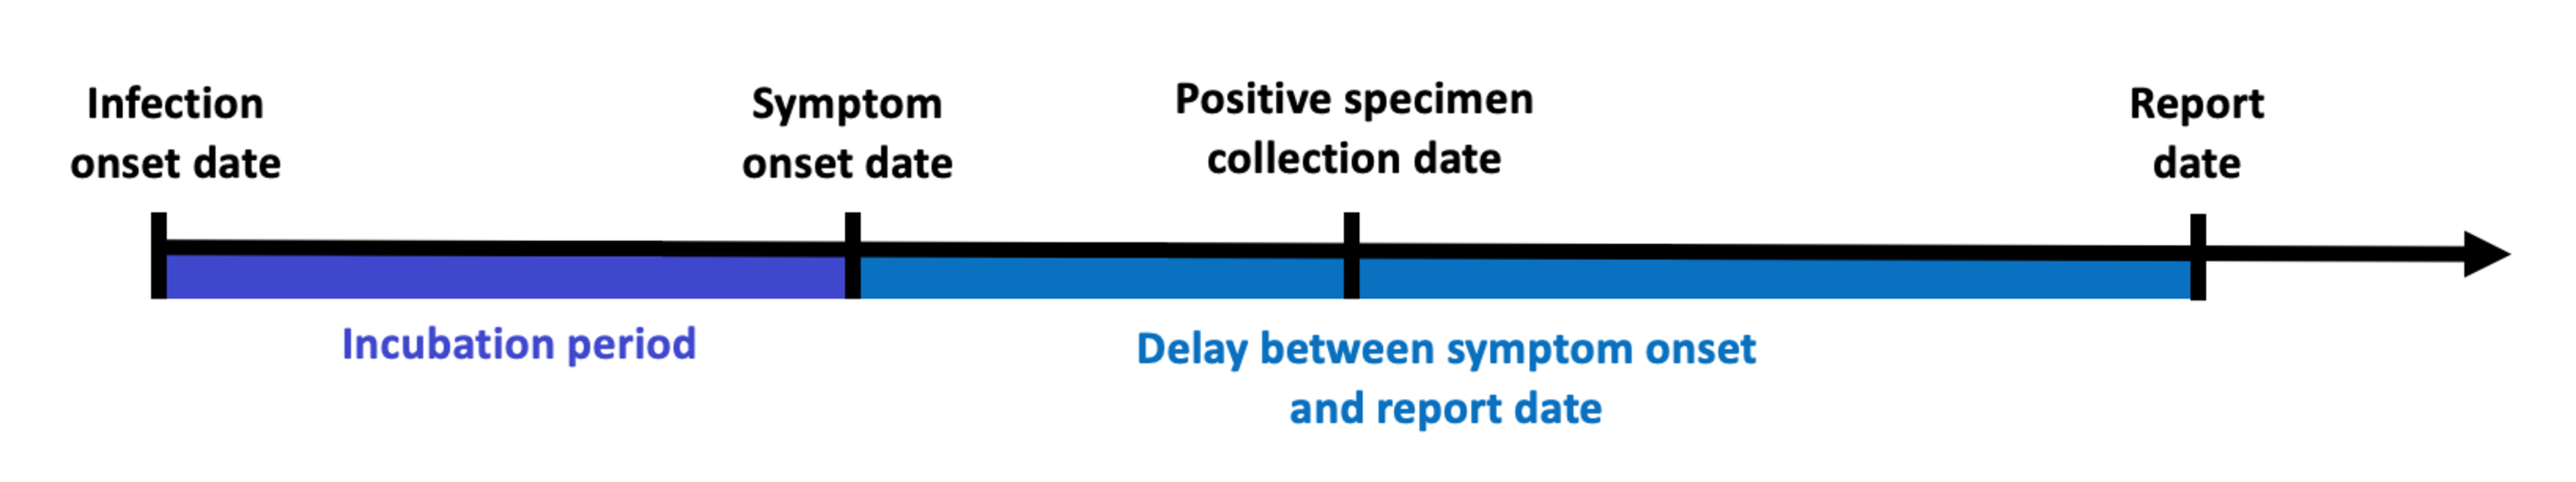
\includegraphics[width=.99\textwidth]{Chain_of_events_onset_report.pdf} 
    \caption{Idealized chain of events from infection onset to case report date 
    for a symptomatic infection that is eventually reported to public health.}
    \label{fig:chain_events_onset_report}
\end{figure}

% Importantly, all of these issues that are present in local health authority
% data are also present in the gold standard for case data from the JHU CSSE
% \citep{dong2020interactive, guidotti2022worldwide} because JHU scrapes case
% data from the local health authority dashboards \citep{jahja2022real}.
% Furthermore, the cases shown on the JHU CSSE Coronavirus Resource Center
% \citep{jhucsse2020covid} are those that have been disseminated to the public
% on a given day. 
% Our approach to estimate latent infections takes case data and estimates the 
% following...

Explaining the course of the pandemic and investigating the effects of
interventions, the burden facing various subgroups, and drawing insights for
future pandemics is inhibited because the true spatial and temporal behaviour of
infections is unknown. While reported cases provide a convenient proxy of the
disease burden in a population, it is incomplete, delayed, and understates the
true size of the pandemic. Regardless of these difficulties, it is important to
the public and public health to perform a pandemic post-mortem and try to better
explain its implications---to attempt to capture the true size and impact of the
pandemic as much as we can. Estimates of daily incident infections are one such
way to measure this and can guide understanding of the pandemic burden over
space and time.

In this work, we provide a statistically rigorous, data-first reconstruction of
daily incident infections for each \US state from June 1, 2020 to November 29,
2021. Using state-level line list data, we construct time-varying delay
distributions for the time from symptom onset to positive specimen date and
positive specimen to case report date. We combine these with variant-specific
incubation period distributions to deconvolve daily reported COVID-19 cases back
to their infection onset. Finally, the resulting deconvolved cases are adjusted
to account for the unreported infections using seroprevalence and reinfection
data to estimate adjust for the waning of antibody detectability over time. We
examine some features of our infection estimates and the implications of using
them rather than reported cases in assessing the impact of the pandemic. We
produce simple time-varying infection-hospitalization ratios (IHRs) for each
state and compare those to similarly derived case-hospitalization ratios (CHRs).
While these analyses provide a glimpse into the utility of our infection
estimates, we believe that there is much more to be explored, and we hope that
our work (and the resulting publicly-available estimates) will prove an
important benchmark for others to undertake retrospective analyses.




\section{Results}
\label{sec:results}

An important aspect of our methods is that deconvolution is not the same as a
shift. \attn{We need a concise description of this somewhere, possibly with a
graphic.}


\subsection{Infection estimates reveal waves missed by reported cases}
\label{sec:omitted-waves}

Outbreaks in infections precede those in reported cases and are reliably larger
in magnitude. But simply shifting cases back in time and increasing them by some
factor fails to capture the spatio-temporal dynamics of the pandemic. 
Hence, relative to reported cases, examining estimated infections reveals a
rather different pattern. \autoref{fig:state_infect_est} shows
estimates of the number of daily new infections per 100,000 inhabitants for each
\US state from June 1, 2020 to November 29, 2021 compared with reported cases,
and deconvolved cases (reported cases ``pushed back'' by the delays shown in
\autoref{fig:chain_events_onset_report}). 

While the major Ancestral, Alpha, and Delta waves tend to be visible for most
states, there are clear outbreaks in unreported infections that are not easily
detectable from cases alone in the falls of 2020 and 2021. For example, a wave 
of infections is present in the spring of 2021 for North Dakota and South Dakota
which is not visible in reported cases alone. \attn{we should search for more of
these patterns.}

\subsection{Spatial-temporal implications are ignored}
\label{sec:ignored-patterns}

\attn{We need to expand the discussion of this figure along the lines we
discussed in our meeting. Choose the dates carefully to emphasize that the
spatial extent during peaks/troughs of waves is different if you look at
infections instead of cases.}

\autoref{fig:choro_inf_case_rates} shows that for the
earliest time of June 1, 2020, there is little discrepancy between case and
infection rates, while for the later times there are immense differences in the
rates, such that case rates tend to underrepresent infections to a great extent.



\subsection{Infection/case ratios vary by state and VOC}
\label{sec:case-infection-ratio}

\attn{The rest of this section uses a lot of space to say, basically, that
infections are bigger than cases. I think we should cut much of it (though see
also below). I think a
better use is to more explicitly emphasize how the case/infection ratio changes
with time and VOC. Let's make that more focused, direct. Note that this isn't
really ``underreporting'', they're still reporting all the tests, but those
tests capture different numbers of infections.}

With respect to variants of concern, consider the late 2020
Ancestral wave for the midwestern states of Illinois, Indiana, and Ohio. For the
major Delta wave, some of the greatest discrepancies between cases and
infections are visible in the western states of Idaho and Montana, the southern
states of Louisiana and Georgia, and the midwestern states of Iowa and Nebraska
(\autoref{fig:state_infect_est}). Earlier on in the pandemic, such discrepancies
between cases and infections may be more attributable to failures in the
reporting pipeline, while later on in the pandemic, they more likely due to the
rise in asymptomatic infections across variants \citep{oph2022covid,
garrett2022high}. 

Finally, while the main Delta wave is somewhat evident from the case counts for
all states (\autoref{fig:state_infect_est}), our estimates suggest that case
counts tend to severely underestimate infections during this time for many
states. The lowest of all states was in New Jersey, where about $4.6\%$ (95\%
confidence interval: $[1.9, 67.7]$) of the estimated infections were reported.
This was followed by Maryland with $7.4\%$ ($[2.7, 83.8]$), Connecticut with
$8.0\%$ ($[3.1, 25.8]$), and Florida with $8.7\%$ ($[4.8, 34.0]$). This
underreporting issue extends to most states as in $39$ states less than $30\%$
of infections were reported during this time. Only $4$ states of Alaska, Maine,
Vermont and Virginia reported at least $40\%$ infections. No states were found
to surpass $50\%$ for reported infections for this time.

Similar patterns were observed during the earlier period of Alpha domination,
where Louisiana had the lowest reported infections at $11.7\%$ (95\% confidence
interval: $[6.7, 31.5]$) and was followed by California at $14.4\%$ (95\%
confidence interval: $[7.7, 68.2]$). There were $23$ states that reported at
least $40\%$ and $22$ states that reported at least $50\%$ of their infections.

Such patterns were comparatively less apparent during the earlier and larger
period of Ancestral domination, where Ohio and Maryland held the lowest
percentages of reported infections at $22.0\%$ (95\% confidence interval:
$[16.2, 34.0]$) and $22.3\%$ (95\% confidence interval: $[14.8, 40.5]$),
respectively. During this time, $28$ states that reported at least $40\%$ and
$14$ states that reported at least $50\%$ of their infections. 

\begin{figure}[!tb]
    \centering
        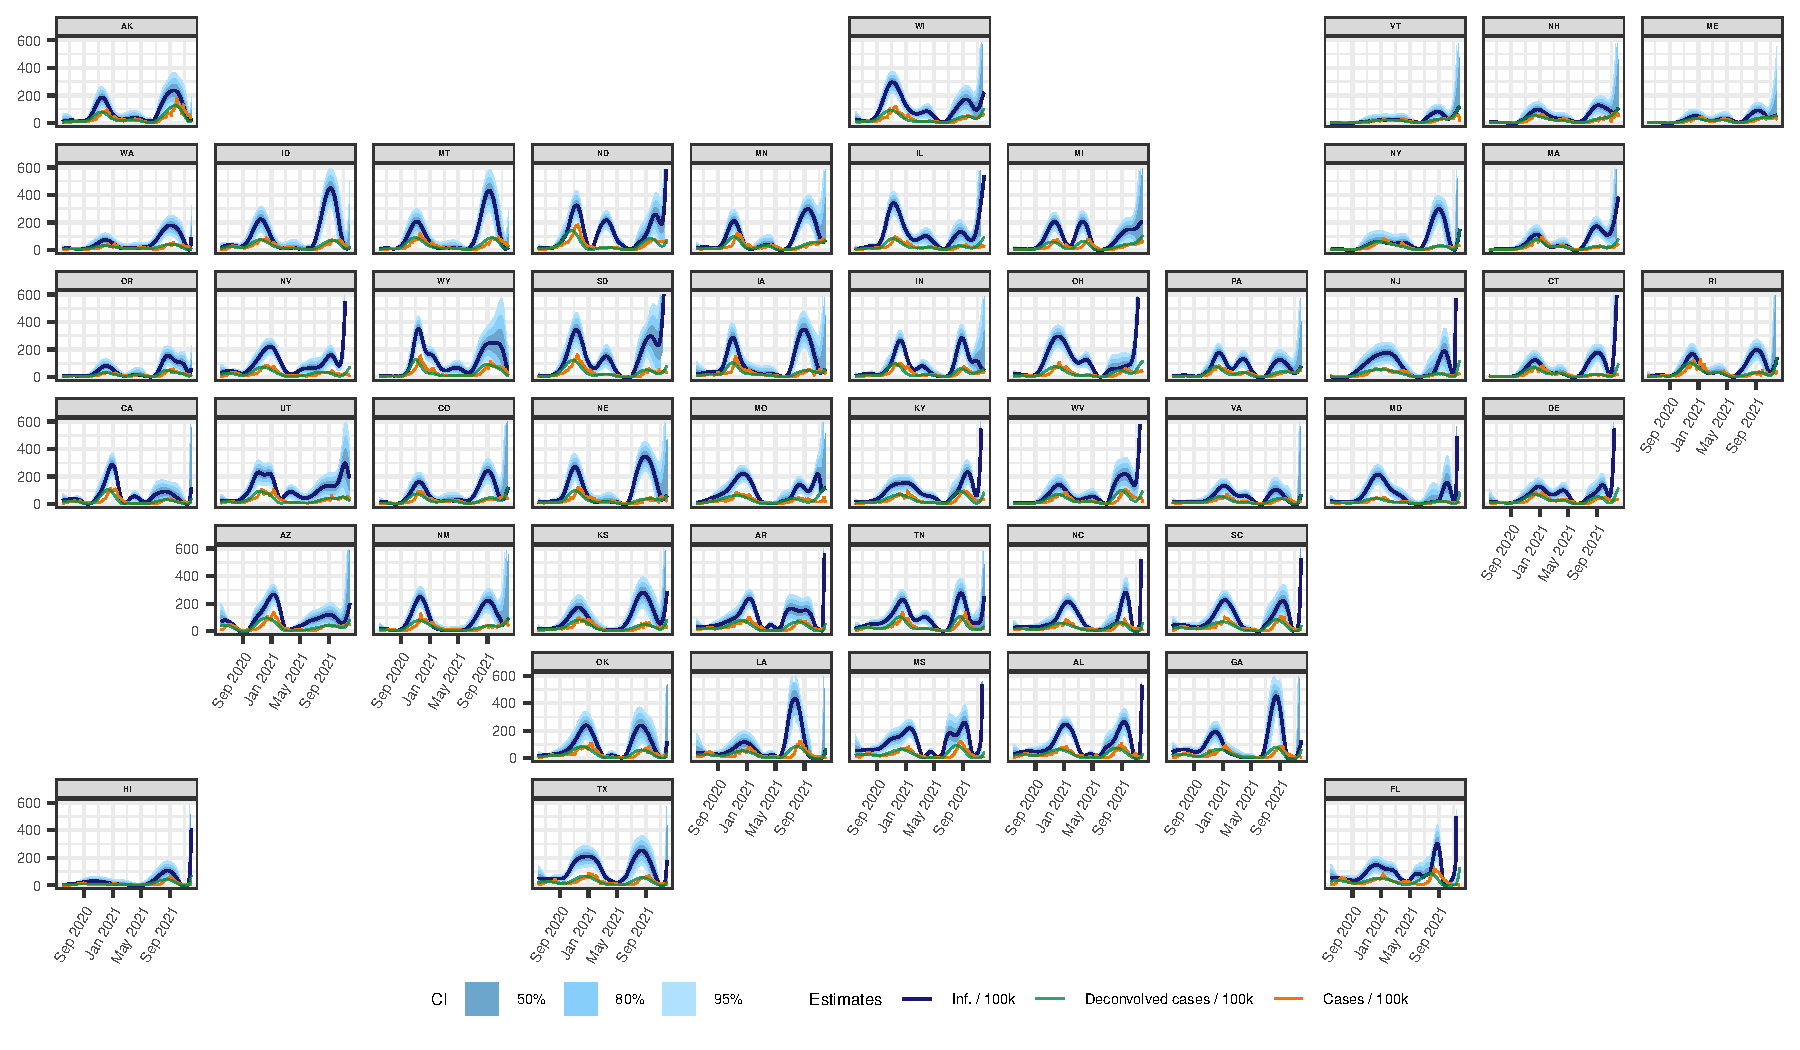
\includegraphics[width=.99\linewidth]{state_niauc_est_faceted_F24.pdf} 
        \caption{Estimates of the number of daily new infections per 100,000
            population for each \US state from June 1, 2020 to November 29, 2021
            (dark blue line). The blue shaded regions depict the 50, 80, and 95\%
            confidence intervals for the estimates, while the teal line represents
            the number of new daily new deconvolved cases per 100,000, and the
            dotted orange line represents the 7-day average of the new cases per
            100,000 as of the same date.}
        \label{fig:state_infect_est}
    \end{figure}
    

\begin{figure}[!tb]
\centering
    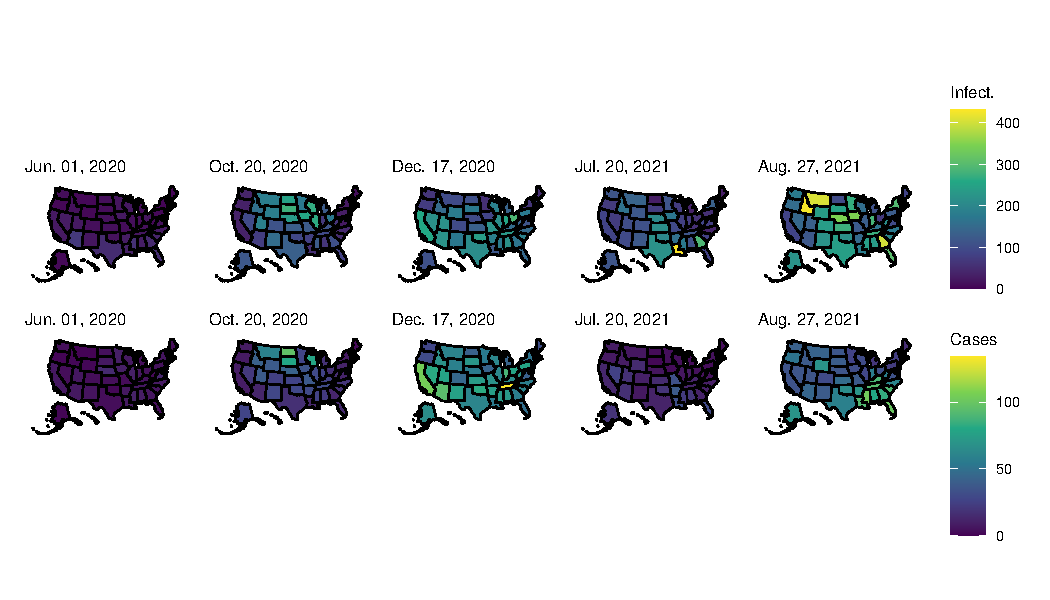
\includegraphics[width=.99\textwidth]{choro_inf_case_rates_F24.pdf}
    \caption{Choropleth maps of the state-level estimates of the number of daily
    new infections per $100,000$ population (top row) and the daily new cases
    per $100,000$ population (bottom row) for three times over the June 1, 2020
    to November 29, 2021 period. The first date was chosen simply as a baseline,
    while the second and third dates were chosen based on the day that had the
    largest number of infections across the 50 states from each year.} 
    \label{fig:choro_inf_case_rates}
\end{figure}    



    
\subsection{Infections broken down by VOCs emphasize earlier outbreaks}
\label{sec:infections-by-voc}

\autoref{fig:six-states} examines the infection estimates for a selection of
states more closely. This set has the largest infection/case ratios. 
\attn{We need to say more about what these 2 figures show, uniquely. What's the
point of looking at them? I think the section heading I wrote is the point. But
we need to say this. The takeaways below are a bit too vague, I think.} The top
panel shows \attn{....} The bottom panel divides estimated
infections into buckets based on the circulating variant proportions at the
time. From these plots, it is clear that few variant categories tends to
dominate and drive infections at a time. The general progression in terms of
variant starts with the Ancestral category from 2020 up to early 2021, to the
Alpha variant in mid 2021, which eventually gets eclipsed by the Delta variant
in mid to late 2021. This supports our division of our results by the three main
variant-driven time periods.


\begin{figure}[!tb]
\centering
    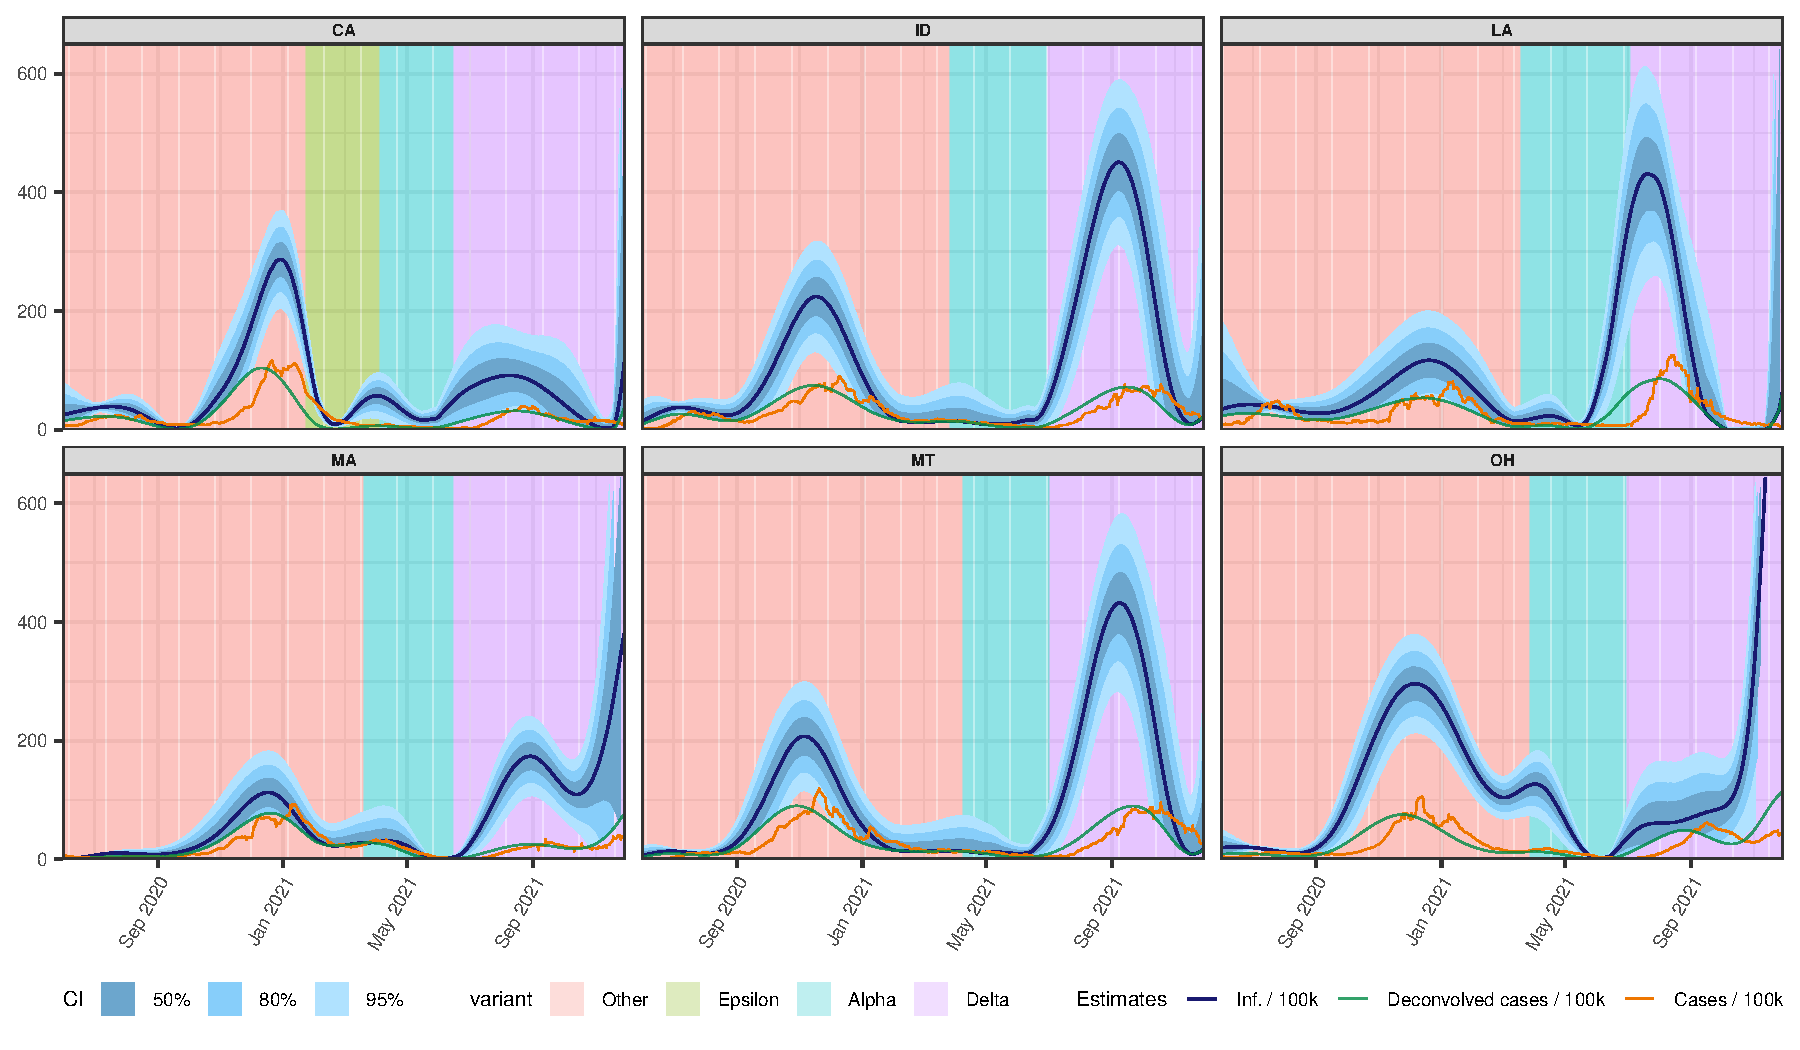
\includegraphics[width=\linewidth]{state_niauc_est_6states_F24.pdf}\\
    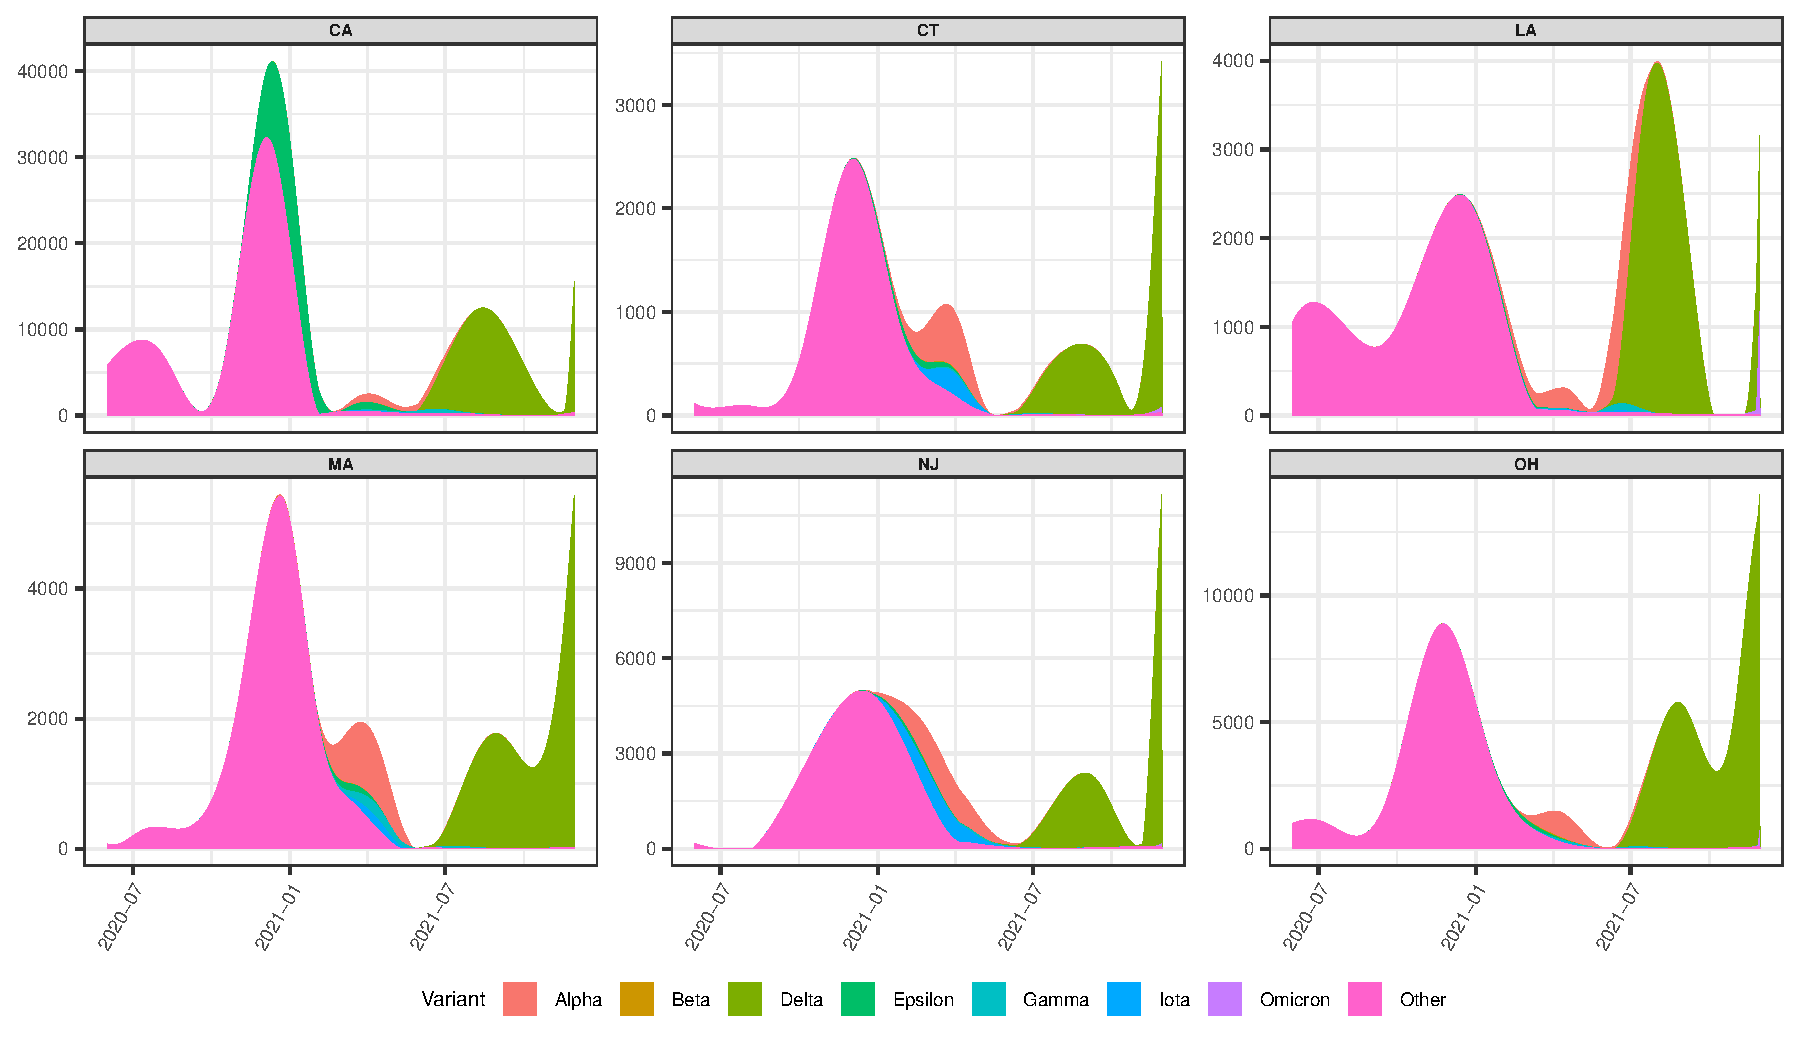
\includegraphics[width=\linewidth]{state_decon_byvar_est_6states_F24.pdf}
    \caption{Top panel: Reported cases, deconvolved cases, and estimates of daily new infections (dark blue
    line) per 100K inhabitants. The blue shaded regions indicate the 50, 80, and 95\% confidence
    bands, while the background is shaded to indicate the dominant variant in
    circulation at the time. \attn{I don't like the rotated x-axis.} 
    Bottom panel: Deconvolved cases colored by variant per 100K inhabitants. \attn{Is
    this the correct units? or are these raw? They should be per 100K.}}
    \label{fig:six-states}
\end{figure}


\subsection{The relationship between infections and hospitalizations is messy}
\label{sec:lagged-correlations}

\attn{messy, but much more stable than CHR} We systematically investigate the
temporal relationship between infections and hospitalizations with Spearman's
rank-correlation across different lags, shifting hospitalizations backward to
align with infections. (\autoref{fig:correlations}). The maximum average
correlation across states is 0.513, occurring at a lag of 13 days. In contrast,
we find that the greatest average Spearman correlation for cases is 0.691 and
occurs at a lag of 1 day. That is, we find that case report rates are nearly
contemporaneous to hospitalizations, while infection estimates clearly precede
them. 

The maximum correlation at a lag of 13 days is in similar to early estimates of the average time from
infection to hospitalization of 9.7 days (95\% CI: $[5.4, 17.0]$) for cases
reported in January, 2020 in Wuhan, China as well as with estimates from across
the pandemic in the UK that ranged from an average of 8.0 to 9.7 days
\citep{ward2021understanding}. 
% However, we should note the first study is based
% on a small sample size for outbreak cases reported well before our study start
% date. As well, both sets of estimates depend upon the healthcare system and the
% population structure, amongst other things \citep{ward2021understanding}.
% Nevertheless, their relative agreement with our estimate of 13 days for the \US
% states lends some credence to of our results. 

\begin{figure}[!tb]
\centering
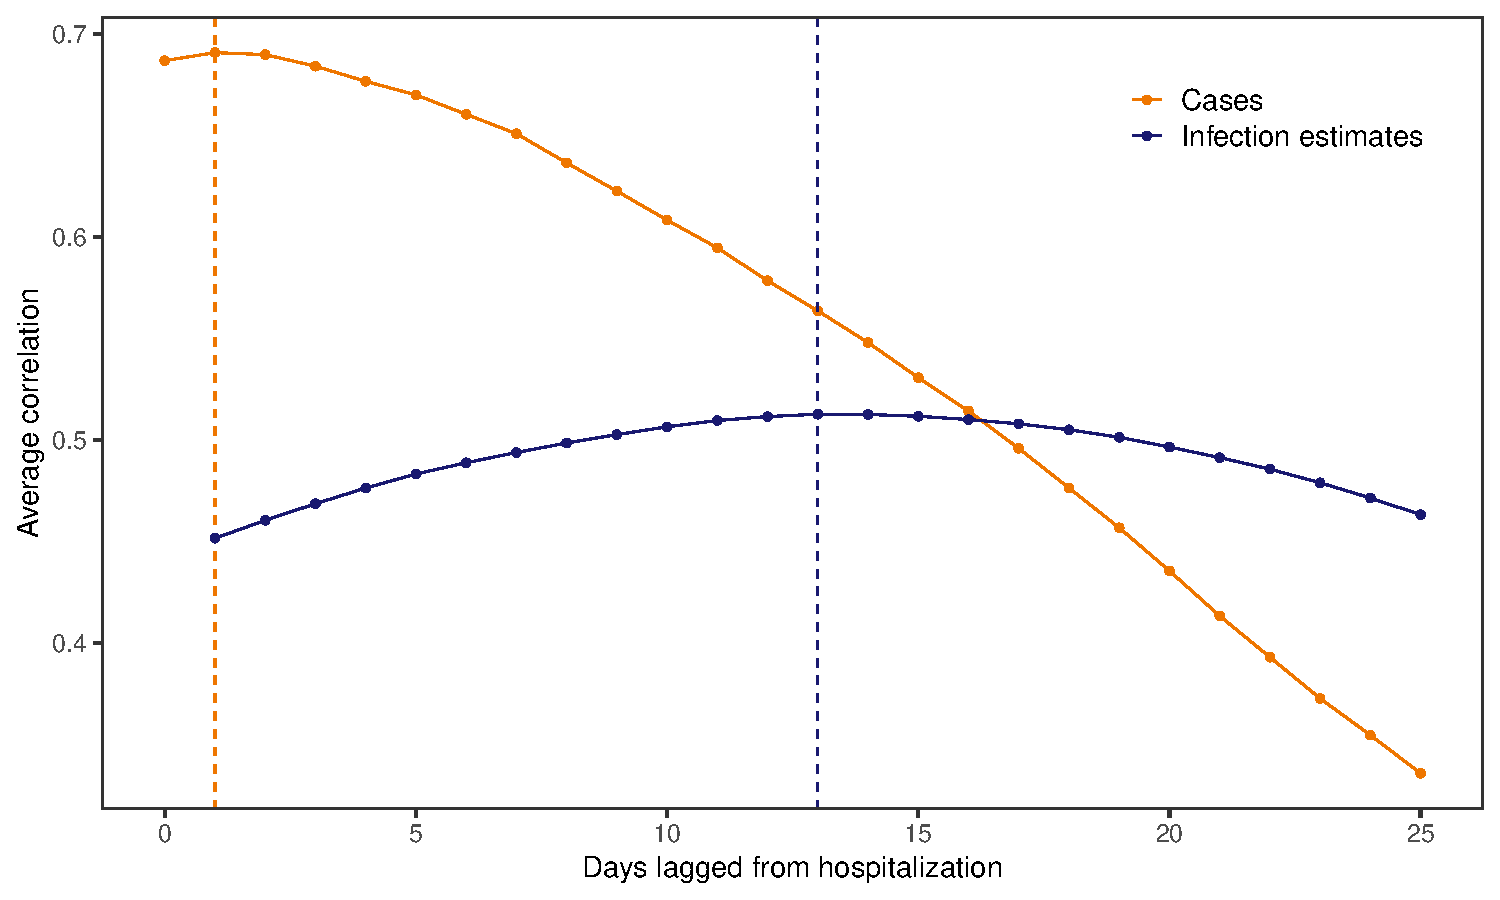
\includegraphics[width=.45\textwidth]{infect_case_hosp_lag_corr_F24.pdf} 
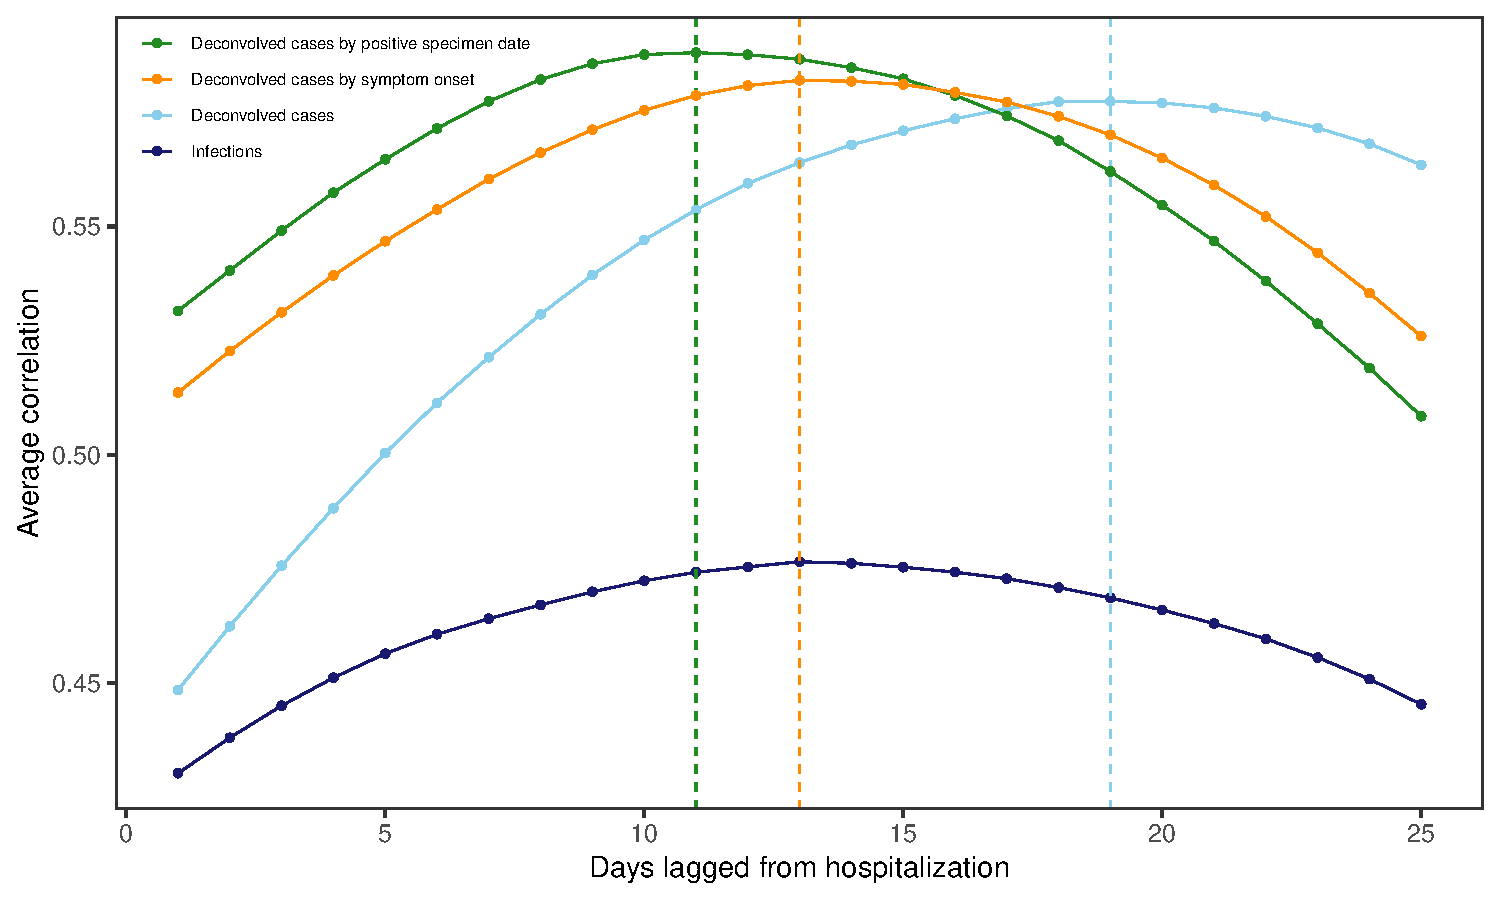
\includegraphics[width=.45\textwidth]{adj_unadj_pi_no_inc_hosp_lag_corr_F24.pdf} 
\caption{Spearman's correlation between the different case/infection ratesand
hospitalization rates per 100,000. These are calculated for each
lag, state and rolling window of 61 days before averaging. 
The vertical dashed lines indicate the lags
for which the highest average correlation is attained. \attn{Let's do one panel
with cases, deconvolved cases, and infections.}}
\label{fig:correlations}
\end{figure}
    

% In terms of the average correlation produced, the deconvolved case estimates by
% infection onset and the deconvolved case estimates by positive specimen date
% reach almost the same maximum average correlation. While that is not a clear
% differentiator by itself, there is a clear time-based benefit of opting for the
% infection estimates by the date of infection onset over symptom onset because
% they provide similar information on hospitalizations about 6 days before the
% latter tends to occur.

Unsurprisingly, the deconvolved case and infection estimates achieve their
maximum correlation at the same lag \attn{I don't think so...}. And yet, the average correlation to
hospitalizations tends to be greater for the deconvolved case estimates than for
the infection estimates. This finding may
stem from a difference in disease severity between the reported and unreported
infections: unreported infections tend to be less severe and less likely to
lead to hospitalization than those that are reported.




\subsection{Estimating infection-hospitalization ratios}
\label{sec:ihrs}

As a counterpart to the correlation analysis, we compute the time-varying
infection-hospitalization ratios (IHRs) for each state using the correlation
maximizing lag. We similarly compute the
case-hospitalization ratios (CHRs) using their correlation maximizing lag for
for comparison (\autoref{fig:IHR_7dav}). 

For each state, the CHRs tend to be larger and noiser relative to
IHRs. This supports our claim that the reported infections are more
likely to require hospitalization than the unreported infections. Both the IHRs
and CHRs exhibit similar geospatial and temporal trends as are noted for
infections. Namely, states that are close in proximity (such as Ohio,
Pennsylvania, and Virginia) tend to exhibit similar patterns in the IHRs and
CHRs over time. In addition, there are similar spikes observed across many
states during waves of infections that are driven by prominent new variants. For
example, many states exhibit a striking spike in hospitalizations in mid-2021,
which coincides with the rapid takeover of the Delta variant during that time
\citep{hodcroft2021covariants}. This finding aligns with previous studies that
found an increased risk in hospitalizations with Delta in comparison to other
variants \citep{twohig2022hospital, nyberg2022comparative}. Similarly, during
the fall of 2020 there tends to be another spike in the IHRs that rivals or
surpasses that observed during the time of Delta (which is the case for states
like New York or Wyoming). 

There does not tend to be a strict upward or downward trajectory or even a
mild waning pattern in the IHRs, as one might expect with later variants that are
more infectious but result in fewer hospitalization
\citep{lorenzo2022covid, blauer2022compare}. Overall, we observe intermittent
spikes that punctuate longer periods where the IHRs tend to stablize slightly below 0.2
hospitalizations per infection. These spikes tend to align with the emergence of
new variants. \attn{0.2 seems wrong. Is the IHR actually H/I? or are the units
not quite right (e.g., H/1M / I/100K)?}

While we computed and compared CHRs and IHRs for all states, it is important to
note that both likely to vary within states and depend on confounding variables
such as age and the presence of major comorbidities
\citep{russell2023comorbidities}. Therefore, it would be beneficial to account
for such variables in their calculations by, for example, stratifying infections
and hospitalizations by age to produce age-specific estimates of the IHRs for
each state~\citep{fox2023disproportionate}.



\begin{figure}[!tb]
\centering
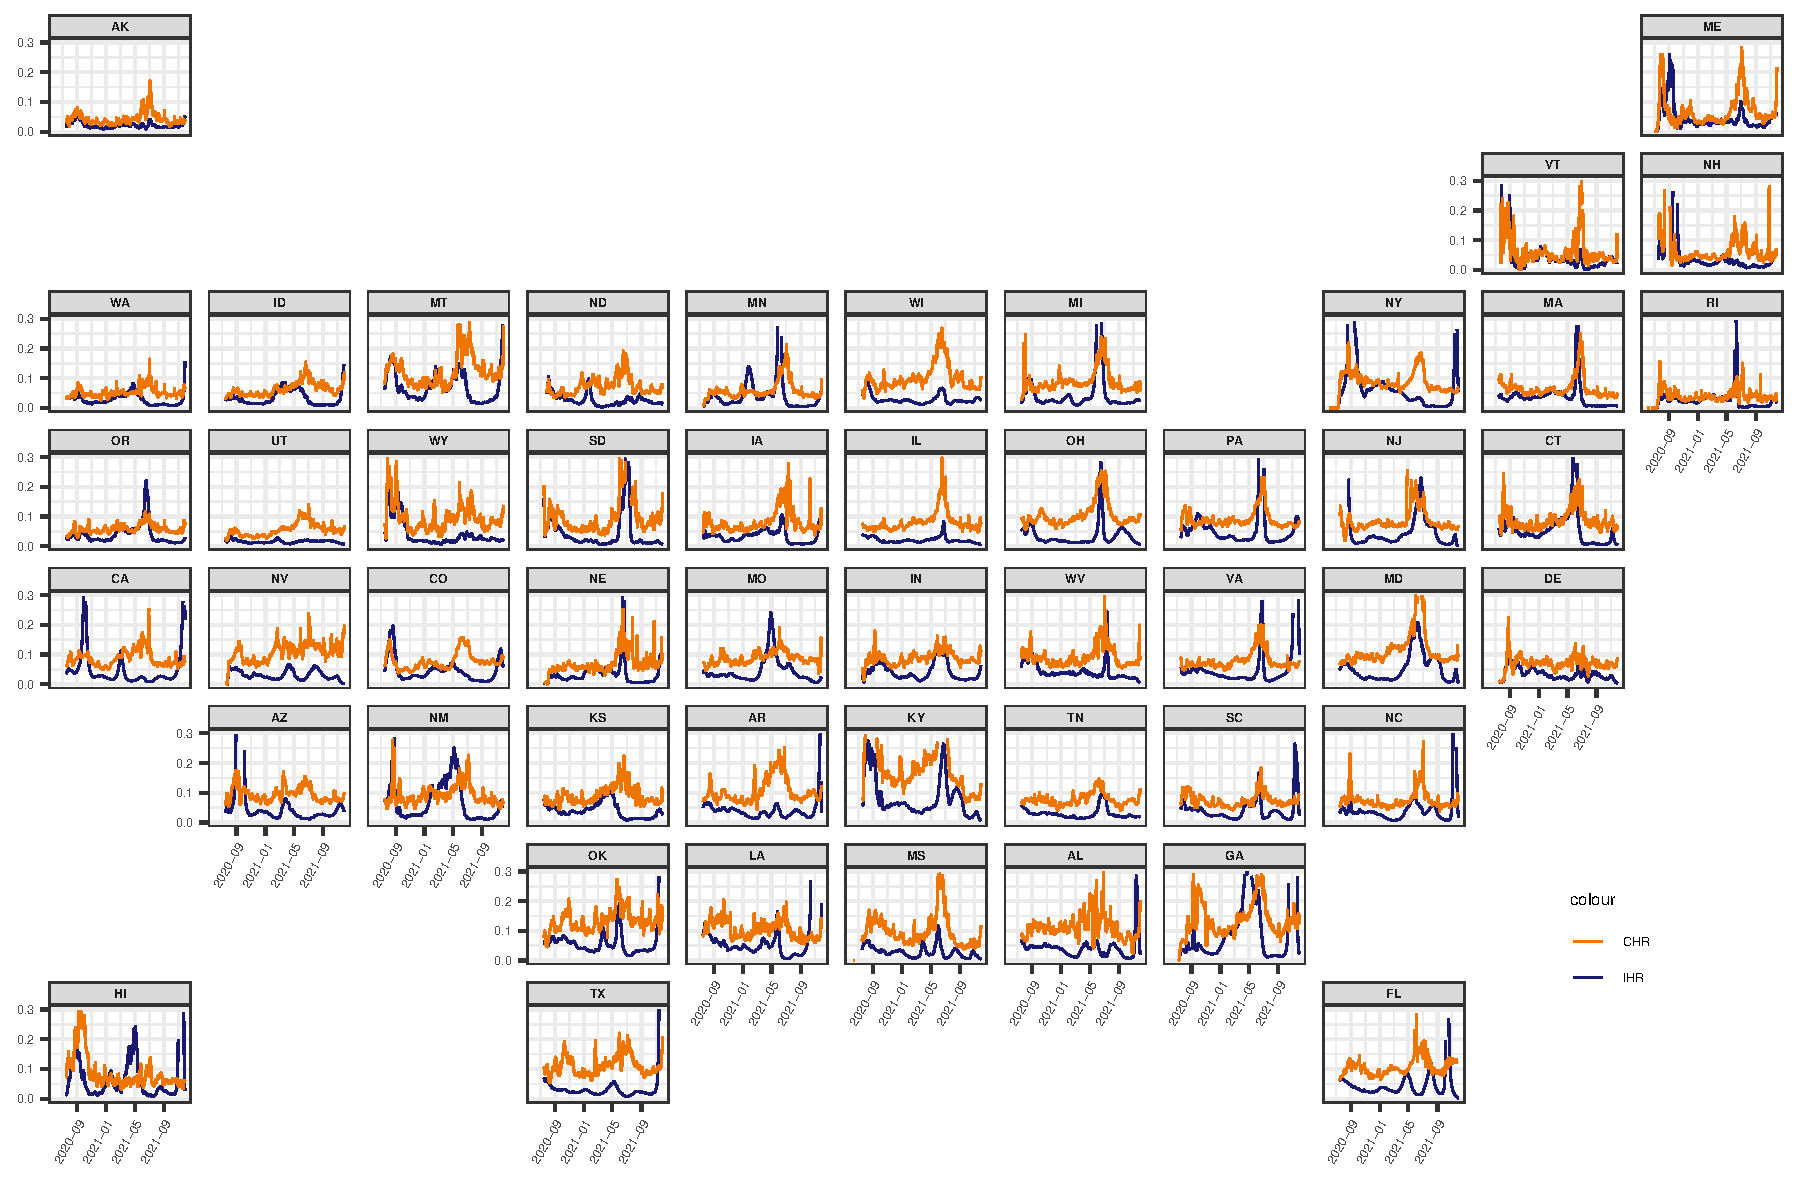
\includegraphics[width=.99\linewidth]{IHR_7dav_F24.pdf}
\caption{Time-varying IHR and CHR estimates for each state from June 1, 2020
to November 29, 2021, obtained using the corresponding optimal lag from the
systematic lag analysis. Note that the infection, case, and hospitalization
counts are subject to a center-aligned 7-day average to remove spurious day
of the week effects. Also note that the different starting points across
states are due to the availability of the hospitalization data.}
\label{fig:IHR_7dav}
\end{figure}


\subsection{Disease burden and viral transmission}

\attn{I'm not yet sure what to do with this. Some of it should go into one of 
the sections above.}

From reconstructing the time series of COVID-19 infections per $100,000$
population for each \US state from June 1, 2020 to November 29, 2021, we
observe rates of infections that vary in intensity and disease burden across
space and time (\autoref{fig:state_infect_est}, \autoref{fig:six-states}).  
Most states present at least two major spikes in infections - the first starts
in the fall of 2020 and extends into the winter season, while the second starts
in the late summer of 2021 and proceeds into the mid-fall. These represent major
waves driven by the Ancestral and Delta variants. Similar patterns in the major
surges of infections are observed in nearly all states, though to varying
degrees. In general, greater similarities in the strength and magnitude of
outbreaks are found to emerge in the clusters of states that border each other.

To avoid encroaching upon possible boundary issues with ending the estimation
during a time of volatility (the period of the Delta-Omicron transition), we
focus on the infection estimates prior to November 1, 2021. The largest observed
outbreaks prior to this time were observed in the late summer or early fall of
2021 in Georgia, Louisiana, Idaho, Montana, and Wyoming which suggests a similar
spread of the virus in small clusters of states that are in close geographic
proximity. During this time, the two states that have the attain the highest
rate of infections per 100,000 on single day are Georgia with about $451$
infections per 100,000 on August 15, 2021 (95\% confidence interval: $[334,
567]$) and Idaho with $451$ on September 7, 2021 (95\% confidence interval:
$[312, 590]$). These are closely followed by Montana with $432$ on September 8,
2021 (95\% confidence interval: $[282, 581]$), Louisiana with $431$ on July 20,
2021 (95\% confidence interval: $[252, 610]$), and Wyoming with $350$ on
November 13, 2020 (95\% confidence interval: $[256, 444]$).

Prior to the Delta wave, the state that has the highest rate of infections per
100,000 on single day is Louisiana with about 358 infections per 100,000 on July
3, 2021 (95\% confidence interval: $[177, 539]$), followed by Wyoming with 349
on November 13, 2020 (95\% confidence interval: $[407, 546]$), South Dakota with
342 infections per 100,000 on July 3, 2021 (95\% confidence interval:$[177,
539]$), and Illinois with 340 infections per 100,000 on July 3, 2021 (95\%
confidence interval: $[177, 539]$). During this time, 74\% of the top rates for
each state were observed in the late fall or winter of 2020.

The period of lowest viral transmission is observed in the summer and fall of
2020. During this time, the state of New Hampshire achieves the lowest weekly
rate of infections of 0.01 infections per 100,000 for the week of September 13,
2020. In the summer of 2020, Vermont maintains a rate under 10 infections per
100,000 from the week of June 1, 2020 to August 30, 2020, which is the longest
continuous stretch observed for any state.

From a brief inspection of the geo-contiguous states, we can observe similar
patterns in surges and periods of waning over time, suggesting that states who
share similarities in climate and topography performed similarly to each other.
More precisely, we can observe neighboring states such as New Hampshire and
Massachusetts or Idaho and Montana that present waves that mirror each other in
amplitude and timing. 

Interestingly, the two states that are geographically removed from the
contiguous United States, Alaska and Hawaii, tend to perform quite differently
from each other later in the pandemic. Alaska generally presents significantly
greater rates of infections than Hawaii especially during the Delta era. This
suggests that it is not so much the non-contiguity aspect as it is other
distinguishing factors that lead to lower infection rates.


%\subsection{Sensitivity analysis}
% This section is under construction
%The infection estimates exhibit modest changes under different assumptions about the
%variant-specific incubation periods, the construction of the delay distribution (the
%window size for the considered onset dates), the fraction of new infections over time, and
%the population estimates (see Supplementary Materials Section X). 
% Potentially compare ww a_t ratios over the time period as well (ie. do they fall in the confidence bands for a_t estimates
% from the ss model)?
% \attn {Add a sentence or two about what is meant by modest changes... Did any of these result in noticeably higher or lower (biased) estimates of infections? To what extent (ie. an additional X infections)? For what states?}
% Do these sensitivity analyses + update this link accordingly.

\section{Discussion}

We retrospectively estimated daily incident infections for each \US state over
the period June 1, 2020 to November 29, 2021. Our  estimates suggest both (a)
that the pandemic impacted states earlier and at a larger scale than is
indicated by cases and that (b) examining cases alone hides some spatio-temporal
waves that become apparent by examining infections. We observe outbreaks in
infections that are difficult to detect from cases alone such as the Delta wave
in New Jersey, Connecticut, and Maryland. This suggests that cases paint an
incomplete picture of the pandemic, especially when outbreaks are largely driven
by unreported infections. Furthermore, since case reports generally follow
symptom and infection onsets, cases have a built-in temporal bias. This is in addition
to other biases from differences in reporting across states (such as temporary
bottlenecks due influxes of data or more persistent processing issues that
increase the average time from case detection to report \citep{wash2020dash,
dunkel2020covid19}. 
% Furthermore, no indication of uncertainty is provided for
% even the gold standard case estimates \citep{delphiepidata2020}. 
Thus, while reported cases provide an indication of the trajectory of the
pandemic, it is a delayed and incomplete version.

% Since case reporting is not
% consistent across time and states, case counts underestimate the true number of
% infections and, hence, the impact of the pandemic \citep{cdc2022estimated,
% simon2022inconsistent}. For example, some states report the number of
% individuals tested rather than the numbers of tests performed
% \citep{schechtman2020counting, chitwood2022reconstructing}. Additionally, while
% the definition of a confirmed COVID-19 case tends to be fairly uniform across
% the United States due to general adherence to the CSTE case definitions, state
% reporting standards have been known to vary \citep{cste2020, delphiepidata2020}.
% For instance, there may be inconsistencies across locations if some cases are
% labelled as confirmed based on positive antigen tests instead of PCR tests
% \citep{covidtracking2021}. 
% As well, the definition of a case and related terminology can change
% or evolve over time as more information becomes available.  

% Estimating the new number of infections by symptom or infection onset date would
% more closely align with the definition of incidence as we know it
% \citep{jahja2022real}.



% The remainder of our discussion consists of an in-depth look into the advantages
% and limitations of our approach and of other comparable approaches, followed by
% a high level summary of our work and its major contributions. 

Our approach offers a number of advantages.
% The development 
% of a way of modelling immunity and space-time-specific reporting ratios based on 
% seroprevalence data.
% Similar phrase on line 1268, though we may want to emphasize that point up here.
% To the best of our knowledge, no other modelling approach has been used to 
% reconstruct the infection time series
%for every state over as much of the COVID-19 pandemic as in this study. %%
%Furthermore, 
For instance, we aim to incorporate as much state-specific information as
possible when deriving our estimates. By using state-level case, line list, and
variant circulation data, we are able to construct incubation and delay
distributions that are specific to each state. Time-varying and state-specific
seroprevalence data allows the reporting ratio estimates to similarly vary over
space and time, a departure from existing work \citep{unwin2020state,
uga2020covid19}. Existing approaches that use the delay distribution to generate
infection estimates often only construct one delay distribution that is used for
all states \citep{chitwood2022reconstructing, jahja2022real}. That is, our work
avoids the assumption of geographic invariance, where it is assumed that
all states have the same patterns of delay from symptom onset to case report.
This assumption is
unlikely to be true due to differences in reporting pipelines, pandemic
response, and variants in circulation, among other issues. 

Another limitation of previous approaches to estimate latent infections is
that they do not to account for reinfections. While
reinfections represent a small fraction of total infections until
later in the pandemic, ignoring them means that the
infection-reporting ratio will tend to be underestimated with seroprevalence
data alone. By accounting for these as well as the waning of seropositivity (See
Methods \autoref{sec:waning-immunity}), we more accurately estimate this ratio.
% so they are not absolutely necessary to include in the
% earlier stages of the pandemic. Still, at no stage did infection confer lifelong
% immunity. Rather antibody levels and immunity are known to wane over time. And
% we believe it is important to account for such defining characteristics of the
% virus when tracking infections over time. Therefore, we account for reinfections
% and the waning of detectable antibody levels in our custom antibody prevalence
% model. 
However, we acknowledge that the extent to which each of these are
accounted for could be improved upon in future work. 
Since the waning of immunity is likely to be variant-dependent
\citep{pooley2023durability}, it follows that our model waning parameter may be
better posed as a mixture of parameters for different variants with weights
determined by the proportion of the variants circulating at the time in the
state. Related to this is the issue that newer variants may escape detection
\citep{nih2022assessing, fda2023sars}. While in a retrospective analysis where
finalized data is used this is less likely to be an issue, this could very well
pose a problem for real-time estimates of infections.

Regarding reinfections, a major reason why we chose an end date of November 29,
2021 and ultimately decided to not tread into Omicron territory is because the
Omicron variants come with substantial increase in the risk of reinfection in
comparison to previous variants as Omicron has been shown to have an increased
tendency towards immune escape \citep{wei2024risk, pulliam2022increased,
eythorsson2022rate}. So having quality reinfection data that is representative
of each location under study is of the utmost importance for the Omicron era. 

% While it would be ideal to use confirmed rates over time for each \US state,
% most states do not publicly report reinfection data over the entire time period
% we considered. So we have turned to suspected reinfection data over time for
% Clark County, USA, as that surveillance is among the most detailed and reputable
% that we have found for the United States. Nevertheless, using such localized
% data raises questions of representativeness and the applicability of such
% estimates to Nevada and all other states. Furthermore, this data has no
% information available beyond suspected third infections, which imposes an
% irremediable bias. However, based on the third infection data available there,
% we expect that the probability of being reinfected more than three times is
% likely very low for time frame considered and so the omission of these would
% impact our infection estimates to a minimal extent. 

% The vast majority of issues we encountered when trying to reconstruct the
% infection time series for each state are due to an absence or a lack of data.
% Such is the primary issue we had with the restricted line list. In comparison to
% the number of JHU cases (which we are treating as a gold standard) for the same
% release date, we noted there are about $10$ million cases that are unaccounted
% for in the CDC line list. Moreover, the missingness does not appear to be random
% and uniformly distributed across states. Rather it is unequally distributed,
% suggesting that the dataset is likely biased. However, more information on the
% cases that are missing versus present would be required to determine the extent
% the missing cases led to a nonrepresentative, and therefore, biased sample, and
% could be a topic of further study.

Using seroprevalence data to estimate the case-ascertainment ratio is subject to
a number of issues, and precludes us from pushing the period of analysis past
the Omicron wave in December 2021. While most state-level data suggests that
reinfections still account for less than 20\% of reported cases during Omicron
\attn{cites}, seropositivity rapidly reaches nearly 100\% of the population,
precluding its continued use. Due to these issues,
alternative data sources for
estimating the case-ascertainment ratio is necessary. 
% Intuitively, one might expect that
% leveraging data from multiple sources would likely lead to more accurate and
% stable estimates than those from using one source. 
For example, wastewater surveillance data
is may be complementary to seroprevalence data,
especially when testing is low \citep{mcmanus2023predicting}. However, 
% there has
% been limited success in predicting incidence using such data. The extent that
% wastewater concentration data is a useful in estimating COVID-19 incidence is
% unclear owing to problems with viral occurrence and detectability in wastewater
% that render 
viral detection is inconsistent across locations due to temperature,
per-capita water use, and in-sewer travel time \citep{mcmanus2023predicting,
hart2020computational, li2023correlation}. Sentinel surveillance streams for
influenza-like illness or acute respiratory infection may provide decent proxies
for COVID-19 incidence, especially when testing for mild cases of COVID-19 is
diminishing or has ceased completely. Finally, alternative surveillance streams
(potentially outside of public health) such as those from surveys, helplines, or
medical records could potentially be integrated if they provide at least a rough
indication of the disease intensity over time
\citep{reinhart2021open,ecdc2020strategies}.



% \attn{Some into Methods, some into Supplement}
% also runs the risk of being nonrepresentative of the
% intended population \citep{bajema2021estimated}. For example, in the blood donor
% dataset some states have region specific-estimates, which clearly do not stand
% for the entire state. Another source of systematic variation is in the
% characteristics of the individuals who opt for blood tests versus those who do
% not. For instance, there may be a healthy user bias, in which a number of those
% who opt for blood tests are generally more inclined to partake in proactive
% healthy behaviors (such as checking on basic health markers by taking an annual
% blood test) than those who do not \citep{parsley2018blood}. Alternatively, a
% number of individuals may be recommended for blood tests by their doctors due to
% signs of ill-health (ex. mineral deficiencies or underlying medical conditions).
% The extent that each such bias persists depends on the purpose of the blood test
% and whether it was used as a proactive or reactive medical tool. Since such
% information is unavailable to us, all we can conclude is that participant-driven
% sources of bias impact the seroprevalence samples to an undetermined extent.
% There are additional concerns about the performance of antibody testing for
% individuals with mild or asymptomatic disease as well as about the loss of
% immunity over time \citep{kaku2021performance, seow2020longitudinal,
% ibarrondo2020rapid}.
% 
% In this work, we do not attempt to directly address infection underascertainment
% due to the increase in asymptomatic infections across variants
% \citep{pho2023covid19}. We simply note that this would likely pose a greater
% problem later in the pandemic, particularly after the Delta era
% \citep{fan2022sars}. We hope that such infections would be largely represented
% by the seroprevalence and reinfection estimates, but there is undoubtedly
% increasing reliance on such estimates to be able to do this over time (owing to
% the simultaneous decline in the reporting cadence and the apparent rise in
% asymptomatic infections over time) \citep{oph2022covid, garrett2022high,
% blauer2022reduce, ren2021asymptomatic}. Consequently, there is an increasing
% uncertainty over time that is not captured by the model or the estimates.   


We adopt a relatively simple deconvolution-based approach and devote
much of our efforts to tailoring our approach to the available data. A major
result of this is the development of a way of to model the waning of detectable
antibody levels and space-time-specific reporting ratios based on seroprevalence
data. In a way, our approach is built for the data rather than trying to force
the data to fit to an existing approach. However, our model is only as good as
the quality and the quantity of the data provided to it. In our case, the lack
of data is both a barrier to entry and a continual roadblock. The assumptions we
are required to make as a consequence of this clearly limit the generalizability
and call into question the reliability of the results. So while we highlight
some interesting trends and numerical findings, these results are not
definitive, but rather exploratory and intended to stimulate discussion on the
challenging task of estimating infections. Despite these limitations, we are
encouraged by the ability to use routine data to produce sensible estimates of
infections in the United States and the plausibility of the apparent geospatial
and temporal trends. 
 


% Our approach is predicated upon having case, line list, viral circulation, and
% seroprevalence data for each state, all of which are readily available (or
% available upon request in the case of restricted line list data). As a result of
% this, we are able to demonstrate the feasibility of estimating COVID-19
% infections at the state level by using standard sources of data. 

% Our framework is quite versatile as it lends itself to more localized, county or
% community level estimates, or globalized, country-specific estimates.
% Fundamentally, to produce estimates of infections for different geographic
% regions, one would simply need to input the required data and re-run the code
% pipeline. In this way, one could readily adapt our approach to generate
% estimates for the provinces in Canada or the regions in England.

Well-informed, localized estimates of COVID-19 infections over time can help us
to have a more clear and comprehensive understanding of the course of the
pandemic. Such estimates contribute important information on the timing and
magnitude of disease burden for each location and they highlight trends that may
not be visible from case data alone. Therefore, our infection estimates provide
key information for the ongoing debate on the true size and impact of the
pandemic.

\section{Methods}


In what follows, we provide details on how we estimate the daily incident
infections for each state over the considered time period of June 1, 2020 to
November 29, 2021 and the data we used to achieve this. 
% We start with a brief
% introduction to each data source used and follow this with a description of each
% major analysis task in the order they are performed.
\autoref{fig:cases_to_infect_flowchart} provides a visual summary of the data,
analysis tasks, and the relationships between them. The major analysis tasks
this figure aims to convey are as follows: First, we estimate variant-specific
incubation periods and two types of delay distributions for each day over the
considered time period. Next, each incubation period and symptom onset to
positive specimen delay distribution are joined using convolution to obtain
variant-specific infection onset to positive specimen distributions for each
time. Then two types of deconvolution are performed. We first deconvolve from
case report to positive specimen date. We then deconvolve from positive specimen
to report date by variant. The resulting infection estimates are aggregated
across the variant categories, and adjusted to account for the unreported
infections by using state-specific, time-varying seroprevalence data in an
antibody prevalence model. This lets us reach our ultimate goal of obtaining
daily incident infection estimates.
% Then, we can apply these estimates in a
% lagged correlation to hospitalizations to find the ``best'' lag between
% infection and hospitalization rates according to Spearman's rank-based correlation 
% and use this to compute time-varying IHRs for each state. 


\begin{figure}[!tb]
\centering
    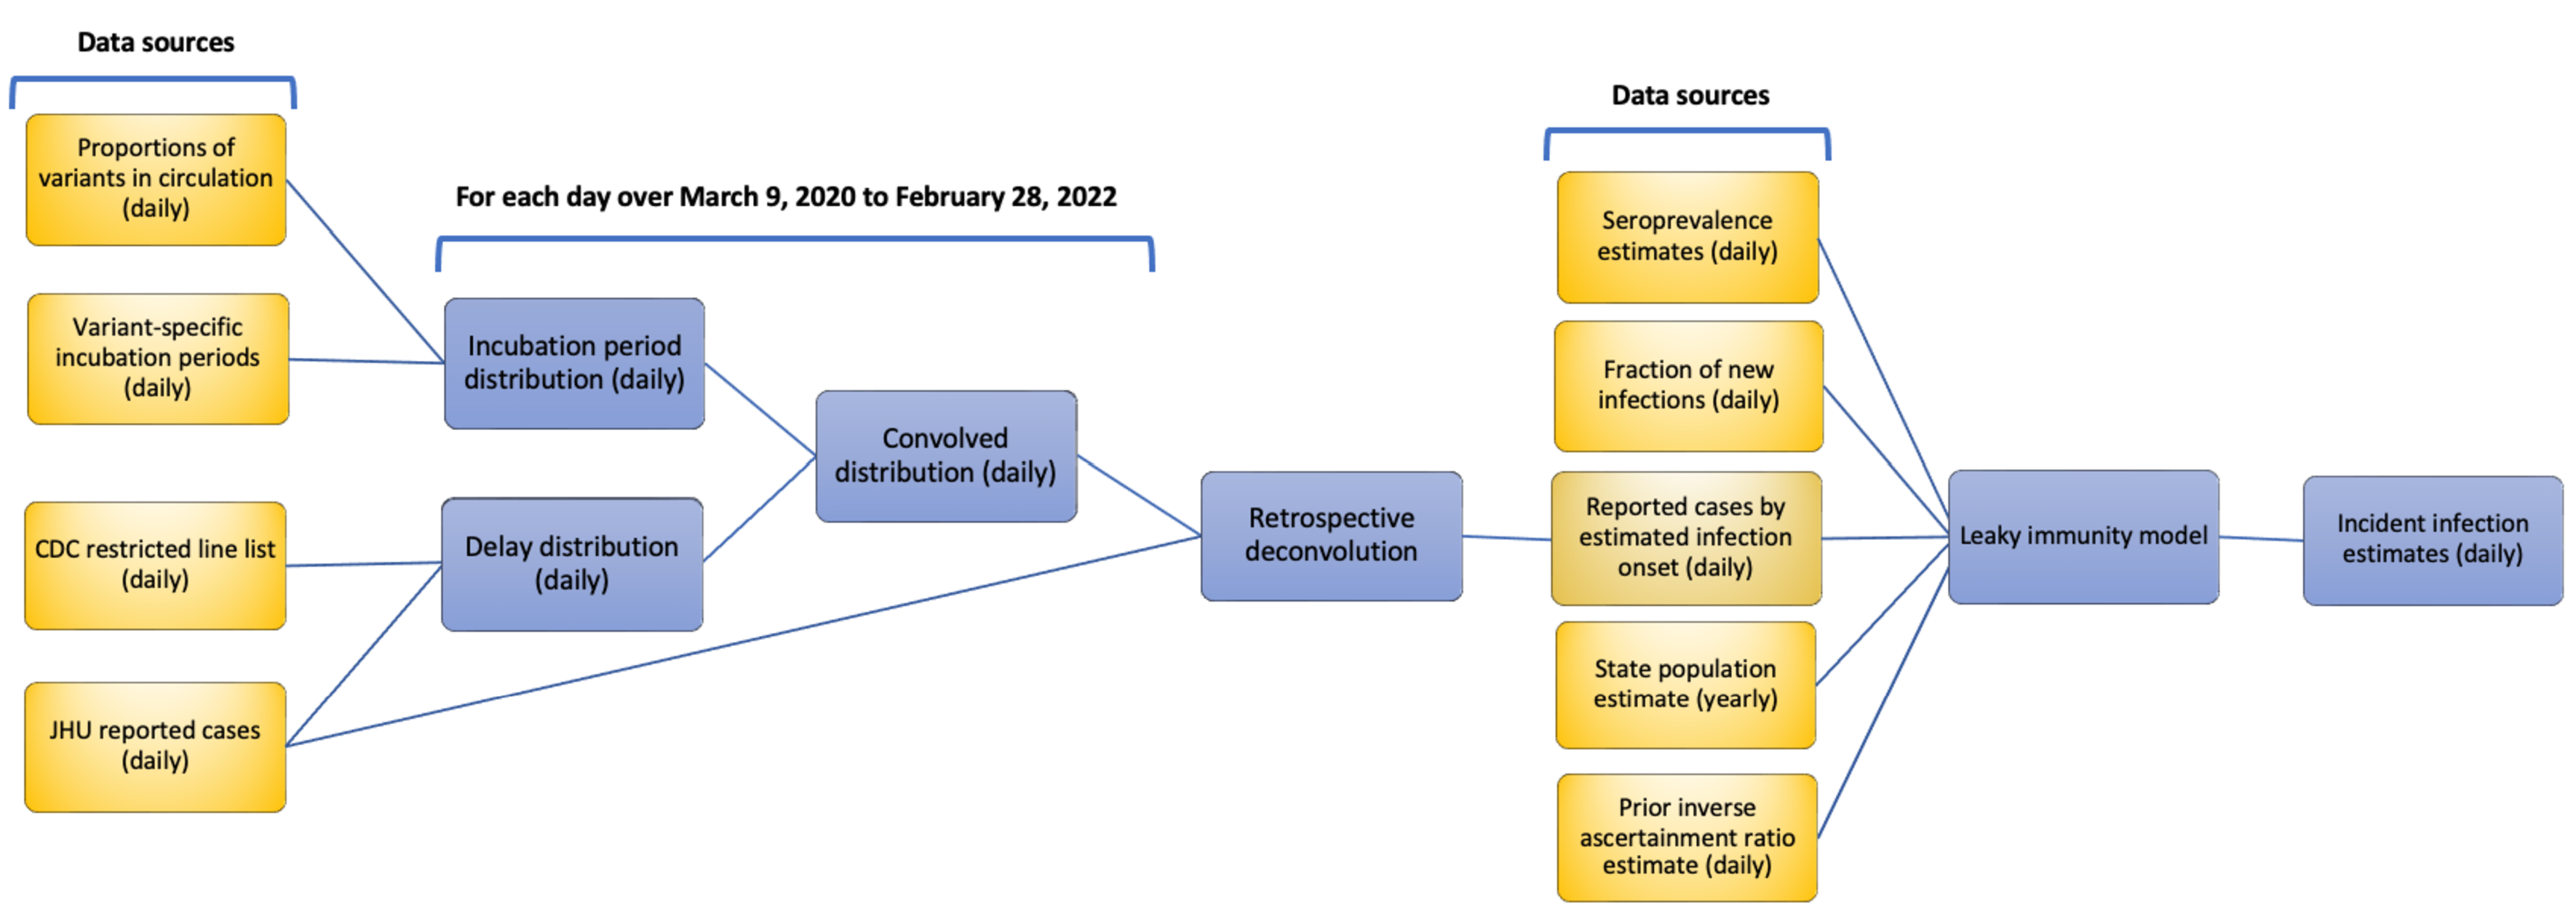
\includegraphics[width=.99\textwidth]{Reported_cases_to_infect_flowchart.pdf} 
    \caption{Flowchart of the inputted data and major analysis steps required 
    to get from reported cases to incident infection estimates for each day 
    over June 1, 2020 to November 29, 2021 for a state. Data sources are coloured 
    in yellow, while data analysis steps are coloured in blue. The data sources that
    do not stem from an analysis step are literature estimates.}
    \label{fig:cases_to_infect_flowchart}
\end{figure}


% Reasons why we should start from June 1, 2020 
% A list of reasons on why I settled on these start and end dates: 
% 1. Reinfections officially started occurring 2020-06-01 according to the data we?re using
% 2. sero measurements start in July 2020 for most states or later
% 3. the prior values for the inverse of the ascertainment ratio estimates are as of 2020-06-01
% 4.  the earliest hospitalizations for each state (that we use in the correlation analysis) 
% are also almost always in July, 2020. 
% So I am not convinced we should extrapolate multiple months away from the start or end for sero. 
% One month in either direction seems reasonable & doesn't overreach.







\subsection{Estimating delay distributions from private line lists}
\label{sec:delaystop}

We obtain de-identified patient-level line list data on COVID-19 cases from the
CDC. Although there are both public and restricted versions of the dataset
available containing the same patient records \citep{cdc2020casepub,
cdc2020caserestr}, only the restricted dataset contains information on the state
of residence. The three key dates of interest are those for symptom onset,
positive specimen collection, and report to the CDC. Handling missingness and
imputation in these dates is somewhat complicated, and additional details and
justifications are deferred to \autoref{sec:linelist-details}.

We use the line list to estimate the delay distribution for the pairs symptom
onset to positive specimen and positive specimen to report. We provide the full
procedure for the latter, before giving a brief description below for the
former. First, define $z_{\ell,t}$ to be a case report occurring at time $t$ in
location $\ell$, and let $\pi_{\ell,t}(k)$ to be the probability that
$z_{\ell,t}$ has a positive specimen collected $k$ days earlier. We assume that
all positive specimens will be reported within 60 days and that no test will be
reported on the same date as it was collected, that is, $\pi_{\ell,t}(0) = 0$
and $\pi_{\ell,t}(k) = 0$ whenever $k > 60$. Let $N_{\ell,t}$ be the number of
$z_{\ell,s}$ with $s\in[t-75+1,t+60] = \mathcal{S}_t$ and positive specimen date
greater than $s-60$. Then, we first compute
\begin{align}
    \tilde{p}_{\ell,t}(k) = \frac{1}{N_{\ell,t}}\sum_{s \in \mathcal{S}_t}
    \big(\textrm{\# $z_{\ell,s}$ with positive specimen at $s-k$}\big).
\end{align}
Next we compute a similar national quantity $\tilde{p}_{t}(k) =
\frac{1}{N_{t}}\sum_{s \in \mathcal{S}_t} \big(\textrm{\# $z_{s}$ with positive
specimen at $s-k$}\big)$, without restricting to location $\ell$. Next, let
$\alpha_{\ell,t}$ be the ratio of $N_{\ell,t}$ to the number of cases reported
by JHU CSSE\cite{dong2020interactive} in the same window. Then, compute
$p_{\ell,t}(k) = \alpha_{\ell,t}\tilde{p}_{\ell,t}(k) +
(1-\alpha_{\ell,t})\tilde{p}_t(k)$. This construction allows for more reliance
on the state estimate when there are more CDC cases relative to JHU (and vice
versa). We calculate the mean $m_{\ell,t}$ and variance $v_{\ell,t}$ of
$\{p_{\ell,t}(k) : 0<k\leq 60\}$ and estimate a gamma distribution by solving
the moment equations $m_{\ell,t} = \alpha_{\ell,t}\theta_{\ell,t}$ and
$v_{\ell,t}= \alpha_{\ell,t}\theta_{\ell,t}^2$ for the shape $\alpha_{\ell,t}$
and scale $\theta_{\ell,t}$. Finally, we discretize the resulting gamma density
to the support set of 1 to 60 days to produce an estimate
$\{\widehat{\pi}_{\ell,t}(k): 0 < k \leq 60\}$ of the delay distribution
$\pi_{\ell,t}$.
 
Estimating the delay from symptom onset to positive specimen date follows the
same procedure with a few minor adjustments. First, we allow $k$ to range from
$-3$ to $21$ (rather than 1 to 60). These upper and lower bounds are based on
the largest delay values for the state-wide 0.05 and 0.95 quantiles. This is
reasonable because the median delay is very short at approximately 2 days, and
an asymptomatic individual may test positive following a known exposure, before
the onset of symptoms. Additional minor details are discussed in
\autoref{sec:delay-justifications}.



\subsection{Estimating the incubation period distributions} 
\label{sec:incubation}

To model the incubation period, the time between infection and symptom onset, we
use estimates from the existing literature, modified slightly to for coherence
with each other: we model each incubation as a gamma distribution with different
parameters. We focus on the following eight variants, which dominated at various
points during our study period: Ancestral, Alpha, Beta, Epsilon, Iota, Gamma,
Delta, and Omicron. Alpha, Beta, Delta, Gamma, and Omicron are all variants of
concern \citep{who2021tracking}, while we include the Epsilon (California) and
Iota (New York) variants because of large impact on those and neighbouring
states \citep{yang2022investigation, duerr2021dominance}.

The Ancestral variant has been modelled as a gamma
distribution~\citep{tindale2020evidence}, so we simply use those reported
parameters. For the Alpha, Beta, Gamma, Delta and Omicron variants, we use the
reported mean and standard deviation of the number of days of incubation
\citep{tanaka2022shorter, grant2022impact, ogata2022shorter}. To match these
moments to the gamma distribution, we solve the same moment equations described
in \autoref{sec:delaystop}. Then, we discretize each resulting density to the support set,
which is taken to be from 1 and 21 days. This range assumes that symptoms
require at least 1 day to develop \citealp{phcan2021covid} and that an
asymptomatic infection will resolve within 21 days \citep{zaki2021estimations,cortes2022sars}.

We were unable to locate incubation period estimates
for the geo-specific Epsilon and Iota variants, so we use the
incubation period for Beta because Epsilon, Iota, and Beta are all children from
the same parent in the phylogenetic tree of the Nextstrain Clades
\citep{hodcroft2021covariants}. All other circulating variants are grouped
together with the Ancestral variant. There was little available sequencing data
prior to Alpha-emergence, but unfortunately, later in the pandemic, it is
impossible to separate Ancestral from other rare variants.

\attn{Perhaps plot the incubation periods? Maybe sharing a panel with the circulation proportions below.}

\subsection{Variant circulation proportions}
\label{sec:variant-proportions}

To estimate the daily proportions of the variants circulating in each state, we
obtain the GISAID genomic sequencing data from CoVariants.org
\citep{hodcroft2021covariants, elbe2017data}. These counts represent the total
number of cases belonging to a particular variant using
a sample of positive tests over a biweekly period. To estimate the population
proportion of each variant, we apply multinomial logistic regression 
for the eight variant categories separately for each state.

We let $V_{j\ell,t}$ to be the probability of a new cases at time $t$ in location
$\ell$ corresponding to variant $j$. Let $v_{j\ell,t}$ be the analogous observed
proportion. Then the nonparametric multinomial logistic regression model is given
as the system
\begin{equation}
\log\left(\frac{V_{j\ell,t}}{1-V_{j\ell,t}}\right) = f_{j\ell}(t),\;\; j=1,\ldots J,\quad
\textrm{subject to }\sum_{j=1}^J \exp\{f_{j\ell}(t)\} = 1, \;\;\forall t.
\end{equation}
The constraint ensures that the estimated proportions will sum to 1 across all
$J$ variants. To encourage smoothness of the estimated proportions, we specify
$f_{j\ell}(t)$ as a third-order polynomial in time: that is $f_{j\ell}(t) =
\beta_{j\ell,0} + \beta_{j\ell,1} t + \beta_{j\ell,2}t^2 + \beta_{j\ell,3}t^3$,
computed such that the resulting matrix of covariates is orthogonal.

\attn{show the result for one
state: the original proportions on the left, and the smoothed on the
right. Then describe this to a small degree (2-3 sentences).}



\subsection{Retrospective deconvolution: from cases to infections}

Retrospective deconvolution estimates the daily number of new infections
corresponding to each variant for each time and location, ``pushing back'' the
dates that those cases were eventually reported to the time of infection.
Because the circulating variant proportions in \autoref{sec:variant-proportions}
correspond to the positive specimen date, this requires two stages. The first is
the deconvolution from report to positive specimen date, and the second is from
positive specimen date to infection onset date.

We will start by describing the first type of deconvolution performed from
report to positive specimen date in detail. For this problem, let $t=1,\ldots,T$
represent the extended deconvolution period from March 1, 2020 to March 1, 2023,
which was chosen to minimize the effects of boundary issues. Define $y_{\ell,t}$
to be the number of new cases reported in location $\ell$ at time $t$, as
reported by the John Hopkins Center for Systems Science and Engineering (JHU
CSSE)\citealp{dong2020interactive} and retrieved with the The COVIDcast API
\citep{reinhart2021open}. Recall that $\widehat{\pi}_{\ell,t}(k)$ is the
associated probability that these reported cases were collected $k$ days earler. 

We estimate the deconvolved cases by positive specimen date by solving the
following optimization problem:
\begin{align}
\minimize_{\mathbf{x}_\ell}\ \sum_{t=1}^T 
\left( y_{\ell,t} -  \sum_{k=1}^{60}\widehat{\pi}_{\ell,t}(k) x_{t-k} \right)^2 
+ \lambda \sum_{t=4}^T \big|x_t - 4x_{t-1} + 6x_{t-2} -4x_{t-3}+ x_{t-4}\big|.
\end{align}
This two parts of this optimization problem trade data fidelity (the sum of
squared errors) with smoothness in the resulting estimates (the absolute error
of the differences of $\mathbf{x}$). The tuning parameter $\lambda$ determines
the relative importance of these competing goals. The solution to the problem is
an adaptive piecewise cubic polynomial \citep{tibshirani2014adaptive,
tibshirani2022divided} and can be accurately computed easily
\citep{ramdas2016fast}. We select $\lambda$ with $3$-fold cross validation
\citep{jahja2022real} in which every third day is reserved for testing, and the
value that results in the smallest out-of-sample mean squared error is chosen.

The result of this first deconvolution is $\widehat{x}_{\ell,t}$, case estimates
by positive specimen date for each state. To continue, pushing back to infection
estimate, we first need the variant-specific delays from infection to positive
specimen collection. These are calculated by convolving the
location-time-specific symptom-to-test distributions from
\autoref{sec:delaystop}, denoted by $\{q_{\ell,t}(k) : -3\leq k \leq 21\}$, with
the variant-specific incubation periods from \autoref{sec:incubation}, denoted
by $\{i_{j}(k) : 0 < k \leq 21\}$. The convolution of these yields a
distribution $\mathbf{q}_{\ell,t}*\mathbf{i}_j = \{\tau_{j\ell,t}(k): -3 \leq k
\leq 42\}$. However, only a fraction of $\widehat{x}_{\ell,t}$ corresponds to
each variant, so we must weight them by the variant proportions
$\widehat{v}_{j\ell,t}$ estimated in \autoref{sec:variant-proportions}. The
analogous optimization problem is therefore:
\begin{align}
\minimize_{\mathbf{u}_{j\ell}}\ \sum_{t=1}^T 
\left( 
    \widehat{v}_{j\ell,t}\widehat{x}_{\ell,t} -  
    \sum_{k=-3}^{42} \tau_{j\ell,t}(k) u_{t-k} 
\right)^2 
+ \lambda \sum_{t=4}^T \big|u_{t} - 4u_{t-1} + 6u_{t-2} -4u_{t-3}+ u_{t-4}\big|.
\end{align}
We call the solution $\widetilde{\mathbf{u}}_{j\ell}$ the \emph{variant-specific deconvolved cases} and
emphasize that these are those cases that will eventually be reported to public
health. Because this deconvolution is done separately for each location and
variant category, we ultimately obtain deconvolved case estimates by the date of
infection onset that are separated by variant. Finally, we will denote the total
deconvolved cases at location $\ell$ as $\widehat{\mathbf{u}}_\ell$.

\subsection{Inverse reporting ratio and the antibody prevalence model} 
\label{sec:report-ratio}

To capture the unreported infections, it is necessary to adjust these deconvolved case estimates by the ratio of the true number of new infections
to the new reported infections. 

Because seroprevalence of anti-nucleocapsid antibodies represents the percentage
of people who have at least one resolving or past infection \citep{cdc2020data},
we can use the change in subsequent seroprevalence measurements to estimate
\emph{all} new infections, rather than just those eventually appearing as cases.
This intuition suggests modelling reported seroprevalence at time $t+1$ as a
fraction $1-\gamma$ of the previous seroprevalence measurement at $t$ plus the
reinfection-adjusted deconvolved cases multiplied by
the inverse reporting ratio at time $t$. That is, 
\begin{align}
s_{\ell,t+1} &= (1 -\gamma_{\ell}) s_t + a_{\ell,t} z_{\ell,t} \widehat{u}_{\ell,t} + \epsilon_{\ell,t},
\end{align}
where $\widehat{u}_{\ell,t}$ is deconvolved cases,
$z_{\ell,t}$ is the percentage of reinfections, $a_{\ell,t}$ is the inverse
reporting ratio, and $\epsilon_{\ell,t}$ represents noise. Note that
$\gamma_{\ell}$ is the percentage of people whose level of infection-induced
antibodies falls below the detection threshold between time $t$ and time
$t+1$. Informally, we refer to $\gamma$ as the waning parameter. Unfortunately,
population seroprevalence is not directly observed, but is measured using
various surveys.

For the proportion of the population in each state with
evidence of previous infection across time, we use two major seroprevalence
surveys: the 2020--2021 Blood Donor Seroprevalence Survey and the Nationwide
Commercial Lab Seroprevalence Survey \citep{cdc2021blood, cdc2021comm}. See
\autoref{sec:sero-details} for additional details. Each of these provides
seroprevalence estimates along with confidence intervals.
The daily fraction of new infections are based on surveillance work conducted by
the Southern Nevada Health District \citep{ruff2022rapid}. \attn{These results
are broadly similar to those in other locations with available data...}

In order to account for different surveys occurring on different dates with
noisy estimates, we estimate the model on the weekly frequency, observed on
Monday, and treat $s_{\ell,t}$ as a latent variable. Therefore, we write,
\begin{align}
\label{eq:waningpr}
r^1_{\ell,m} &= s_{\ell,m} + \tau_{\ell,m}, 
  & \tau_{\ell,m} &\sim \textrm{N}(0,\ w^1_{\ell,m}\sigma^2_r)\\
r^2_{\ell,m} &= s_{\ell,m} + \varphi_{\ell,m}, 
  & \varphi_{\ell,m} &\sim \textrm{N}(0,\ w^2_{\ell,m}\sigma^2_r)\\
s_{\ell,m+1} &= (1 -\gamma_{\ell}) s_{\ell,m} + 
  a_{\ell,m} z_{\ell,m} y^\Sigma_{\ell,m} + \epsilon_{\ell,m}, 
  & \epsilon_{m} &\sim \textrm{N}(0,\ \sigma^2_{\ell,\epsilon}),
\end{align}
where $r^1$ and $r^2$ correspond to the two different seroprevalence surveys.
These surveys each have measurement errors with variance $\sigma^2_r$ that scale
proportional to the observed confidence intervals for the estimates,
respectively $w^1_{\ell,m}$ and $w^2_{\ell,m}$. We denote
$\widehat{u}^\Sigma_{\ell,m} = \sum_{t=m}^{m+1} \widehat{u}_{\ell,t}$. Finally,
to ensure that $\mathbf{a}_\ell$ is smooth over time, we complete the model with
an additional equation that enforces smoothness
\begin{align}
a_{\ell,m+1} &= 3a_{\ell,m} - 3a_{\ell,m-1} + a_{\ell,m-2} + \eta_m, 
  &\eta_m  &\sim \textrm{N}(0, \sigma^2_{\eta}).
\end{align}
    
This antibody prevalence model is a state-space model with latent variables
$\mathbf{s}_{\ell}$ and $\mathbf{a}_{\ell}$ and unknown parameters $\gamma_\ell$,
$\sigma^2_r$, $\sigma^2_\epsilon$, and $\sigma^2_\eta$. This model
allows for convenient handling of missing data, extrapolation
before and after the period of observed seroprevalence measurements, and maximum
likelihood estimates of the errors. Details of this
methodology and the computation of the associated uncertainty measurements are
deferred to \autoref{supp:ssapm}.



\subsection{Lagged correlation to hospitalizations and time-varying IHRs} 

From the same API, we also retrieve the daily number of confirmed COVID-19
hospital admissions for each state that are collected by the \US Department of
Health and Human Services (HHS). Both datasets are updated as of June 6, 2022.

We use our infection estimates in a lagged correlation analysis with confirmed
COVID-19 hospitalizations. Our primary goal of this analysis is to find the lag
between infection and hospitalization rates that gives the highest average
rank-based correlation across \US states. To that end, we consider a wide range
of possible lag values ranging from 1 to 25 days. Zero and negative lags are not
considered because COVID-19 infection onset must precede hospitalization due to
the virus. To remove day of the week effects, both the infection and
hospitalization signals are subject to a 7-day moving average (center-aligned)
before their conversion to rates.

For each considered lag, we calculate the Spearman's correlation between the 
state infection and hospitalization rates for each observed day 
over the June 1, 2020 to November 29, 2021
time period %, and use the epi\_slide function \citep{mcdonald2023epipredict} to 
with a center-aligned rolling window of 61 days for each such computation.
We then calculate the average correlation across all states and times for each lag. 
The lag that leads to the highest average correlation is used to estimate 
the time-varying IHRs for each
state. To compute this for a given day, the number of individuals who are
hospitalized due to COVID-19 on a day are divided by the estimated total number
who were infected on the lagged number of days before.


\section*{Data availability}
\section*{Code availability}

\clearpage
\bibliographystyle{unsrtnat}
\bibliography{bibliography.bib}
%\bibliographystyle{naturemag} %% Change back to numeric references in line with
%requirements for Nature Communications articles (see pg 3 fro here:
%https://www.nature.com/documents/ncomms-formatting-instructions.pdf)



\section*{Acknowledgements}

% Required Gisaid acknowledgement
We gratefully acknowledge all data contributors, i.e., the Authors and their
Originating laboratories responsible for obtaining the specimens, and their
Submitting laboratories for generating the genetic sequence and metadata and
sharing via the GISAID Initiative \citep{elbe2017data}, on which this research
is based.

\attn{Grants, Delphi, etc.}

\section*{Author contributions}

\section*{Competing interests}

The authors declare no competing interests.





\clearpage
% Eventually make the supplement a separate document with its own title page 
\beginsupplement
\title{\supptitlefont Online Supplement}
\maketitle

\section{Additional details on data and methodology}

This section contains additional information about the data used as well as
details about statistical methodology.

\subsection{A general description and depiction of convolution}
\label{supp:convol}

In general, the goal of convolution is to propagate the input signal forward in
time using a probability distribution. In the 1D and discrete context, it is
simply a rolling, weighted average of the past. So for an input sequence
$\{x_t\}_{t=1}^n$ and time-constant weights $\{z(k)\}_{k=-\infty}^0$, the output
sequence $\{y_t\}_{t=1}^n$ is given by
\begin{equation}
    y_t = \sum_{s=0}^t z(s)x_{t-s}.
\end{equation}
\Cref{fig:convol} presents a depiction of the convolution procedure for an
example signal $x_t$ (smoothed cases, orange line). Essentially, to push the
cases forward in time, we take the appropriately aligned (forward-in-time) delay
distribution $z(s)$ (blue shaded region) and convolve it with the smoothed cases
signal counts by it to get the convolved  estimates (blue line). This process is
repeated as we march forward in time, as shown through the stop-motion panels,
such that it eventually covers the entire line of cases. An important takeaway
from this is that convolution is not the same as a simple shift of the data.
A shift is a special case: when $z(d)=1$ and $z(s)=0$, $s\neq d$, we shift $x$
forward by $d$. Rather, convolution generally weights the entire past by
non-zero probabilities. Deconvolution proceeds in the same fashion, but in the
opposite direction, going backward in time and undoing the effect of a
convolution. 

\begin{figure}[H]
\centering
    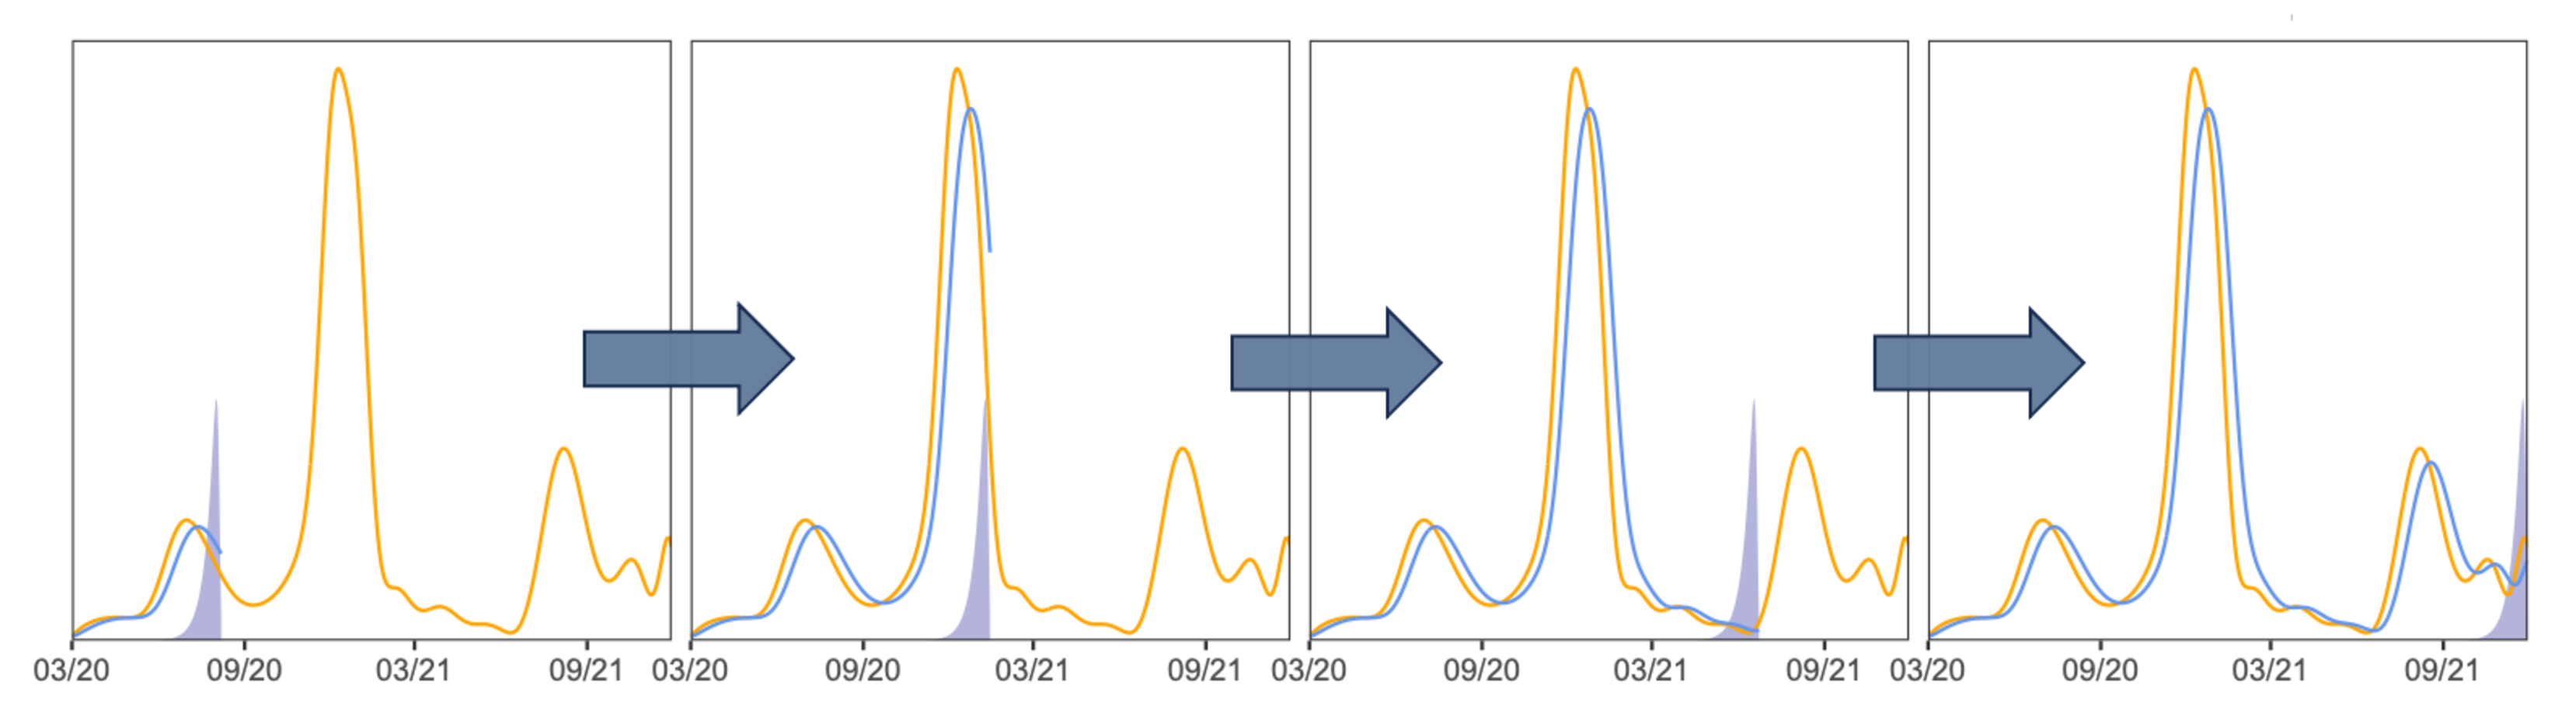
\includegraphics[width=0.99\linewidth]{convolution_diagram.pdf}
    \caption{A general depiction of convolving smoothed cases (orange line) with the corresponding delay probabilities (shaded blue area) to get the convolved estimates (blue line) over four different times.}
    \label{fig:convol}
\end{figure}

\subsection{Additional details on the date fields in the CDC line list}
\label{supp:linelist-details}

Because the CDC line list is updated monthly and cases may undergo revision, we
use a single version of it that was released on June 6, 2022. We consider this
version to be finalized in that it is well-beyond our study end date such that
the dataset is unlikely to be subject to further significant revisions.

\Cref{tab:order-events-table} presents the percent of pairwise occurrences for
the different possible permutations of events in the line list. Essentially,
most cases follow the idealized ordering shown by
\Cref{fig:chain_events_onset_report} and so we adhere to this construction as
much as possible. Unfortunately, the line list has significant missing data,
notably with respect to our variables of interest. Approximately 62.3\% of cases
are missing the symptom onset date, 55.4\% are missing positive specimen date,
and 8.96\% of cases are missing the report date. Furthermore, cases with missing
report or positive specimen dates may be filled with their symptom onset date
\citep{jahja2022real}. So it is possible that all three variables may have the
same date for a case. However, we only actually deal with pairs of these events;
we do not use all three at once in our construction of the delay distributions.
Therefore, we restrict our investigation of coincident missingness to the possible pairs.
% \Cref{fig:prop-cc} suggests that this issue impacts states differentially due to
% the inconsistent proportions of zero delay between positive specimen and report
% date across states. 

\begin{table}[t!]
    \centering
\begin{tabular}{@{}lp{3cm}p{8.5cm}@{}}
\toprule
\textbf{Order of events}& \textbf{Percent pairwise occurrence} &
\textbf{Handling}\\ \midrule \addlinespace
IO $\rightarrow$ SO $\rightarrow$ PS $\rightarrow$ RE & \begin{tabular}[t]{@{}l@{}}PS $\geq$ SO: 97.1 \\ PS = SO: 33.6\\ PS \textgreater\ RE: 1.74\\  PS = RE: 14.6\end{tabular} & This is the idealized order of events and so the  support sets for  SO $\rightarrow$ PS and PS $\rightarrow$ RE delay distribution constructions around this such that IO comes first by construction, SO typically precedes PS, but may be the same  or come before, and RE comes after PS and SO \\ \addlinespace
IO $\rightarrow$ PS $\rightarrow$ SO $\rightarrow$ RE & \begin{tabular}[t]{@{}l@{}}PS \textless\ SO: 2.91 \\ SO $\leq$ RE: 99.3 \\ SO \textless\ RE: 86.1\end{tabular}            & Allowed for negative delays up to the largest non-outlier value for the 0.05 quantile of delay from PS to SO by state                                                                                                                                         \\ \addlinespace
IO $\rightarrow$ PS $\rightarrow$ RE $\rightarrow$ SO & \begin{tabular}[t]{@{}l@{}}RE \textless\ SO: 0.7 \\ RE \textless\ PS: 1.7\end{tabular}                                    & Current handling by the CDC of the line list ensures that the most concerning cases are handled where SO = PO = RE, SO = RE and PO = RE                                                                                                                                                \\ \addlinespace\bottomrule
\end{tabular}
\caption{Percent pairwise occurrence for the different permutations of events considered in the restricted CDC line list. The abbreviation IO stands for infection onset, SO is symptom onset, PS is positive specimen, and RE is report date. We consider a restricted set of permutations because we assume that IO must come first and that PS must precede report date for a case to be legitimate. Finally, the underlying assumption for the percent pairwise occurrence calculations is that the cases must have both elements present (not missing).}
\label{tab:order-events-table}
\end{table}


Due to the contamination in the zero delay cases (those whose symptom onset was
used to fill missing positive specimen or report date, the true extent of which
is unknown to us), we omit all cases where the positive specimen and report
dates have zero delay from our analysis. We choose to allow for zero and
negative delay for symptom onset to report because correspondence with the CDC
confirms the possibility that a person could test positive before symptom onset
and it is a reasonable ordering to expect if, for example, the individual is
aware that they have been exposed to an infected individual.

\begin{figure}[!tb]
\centering
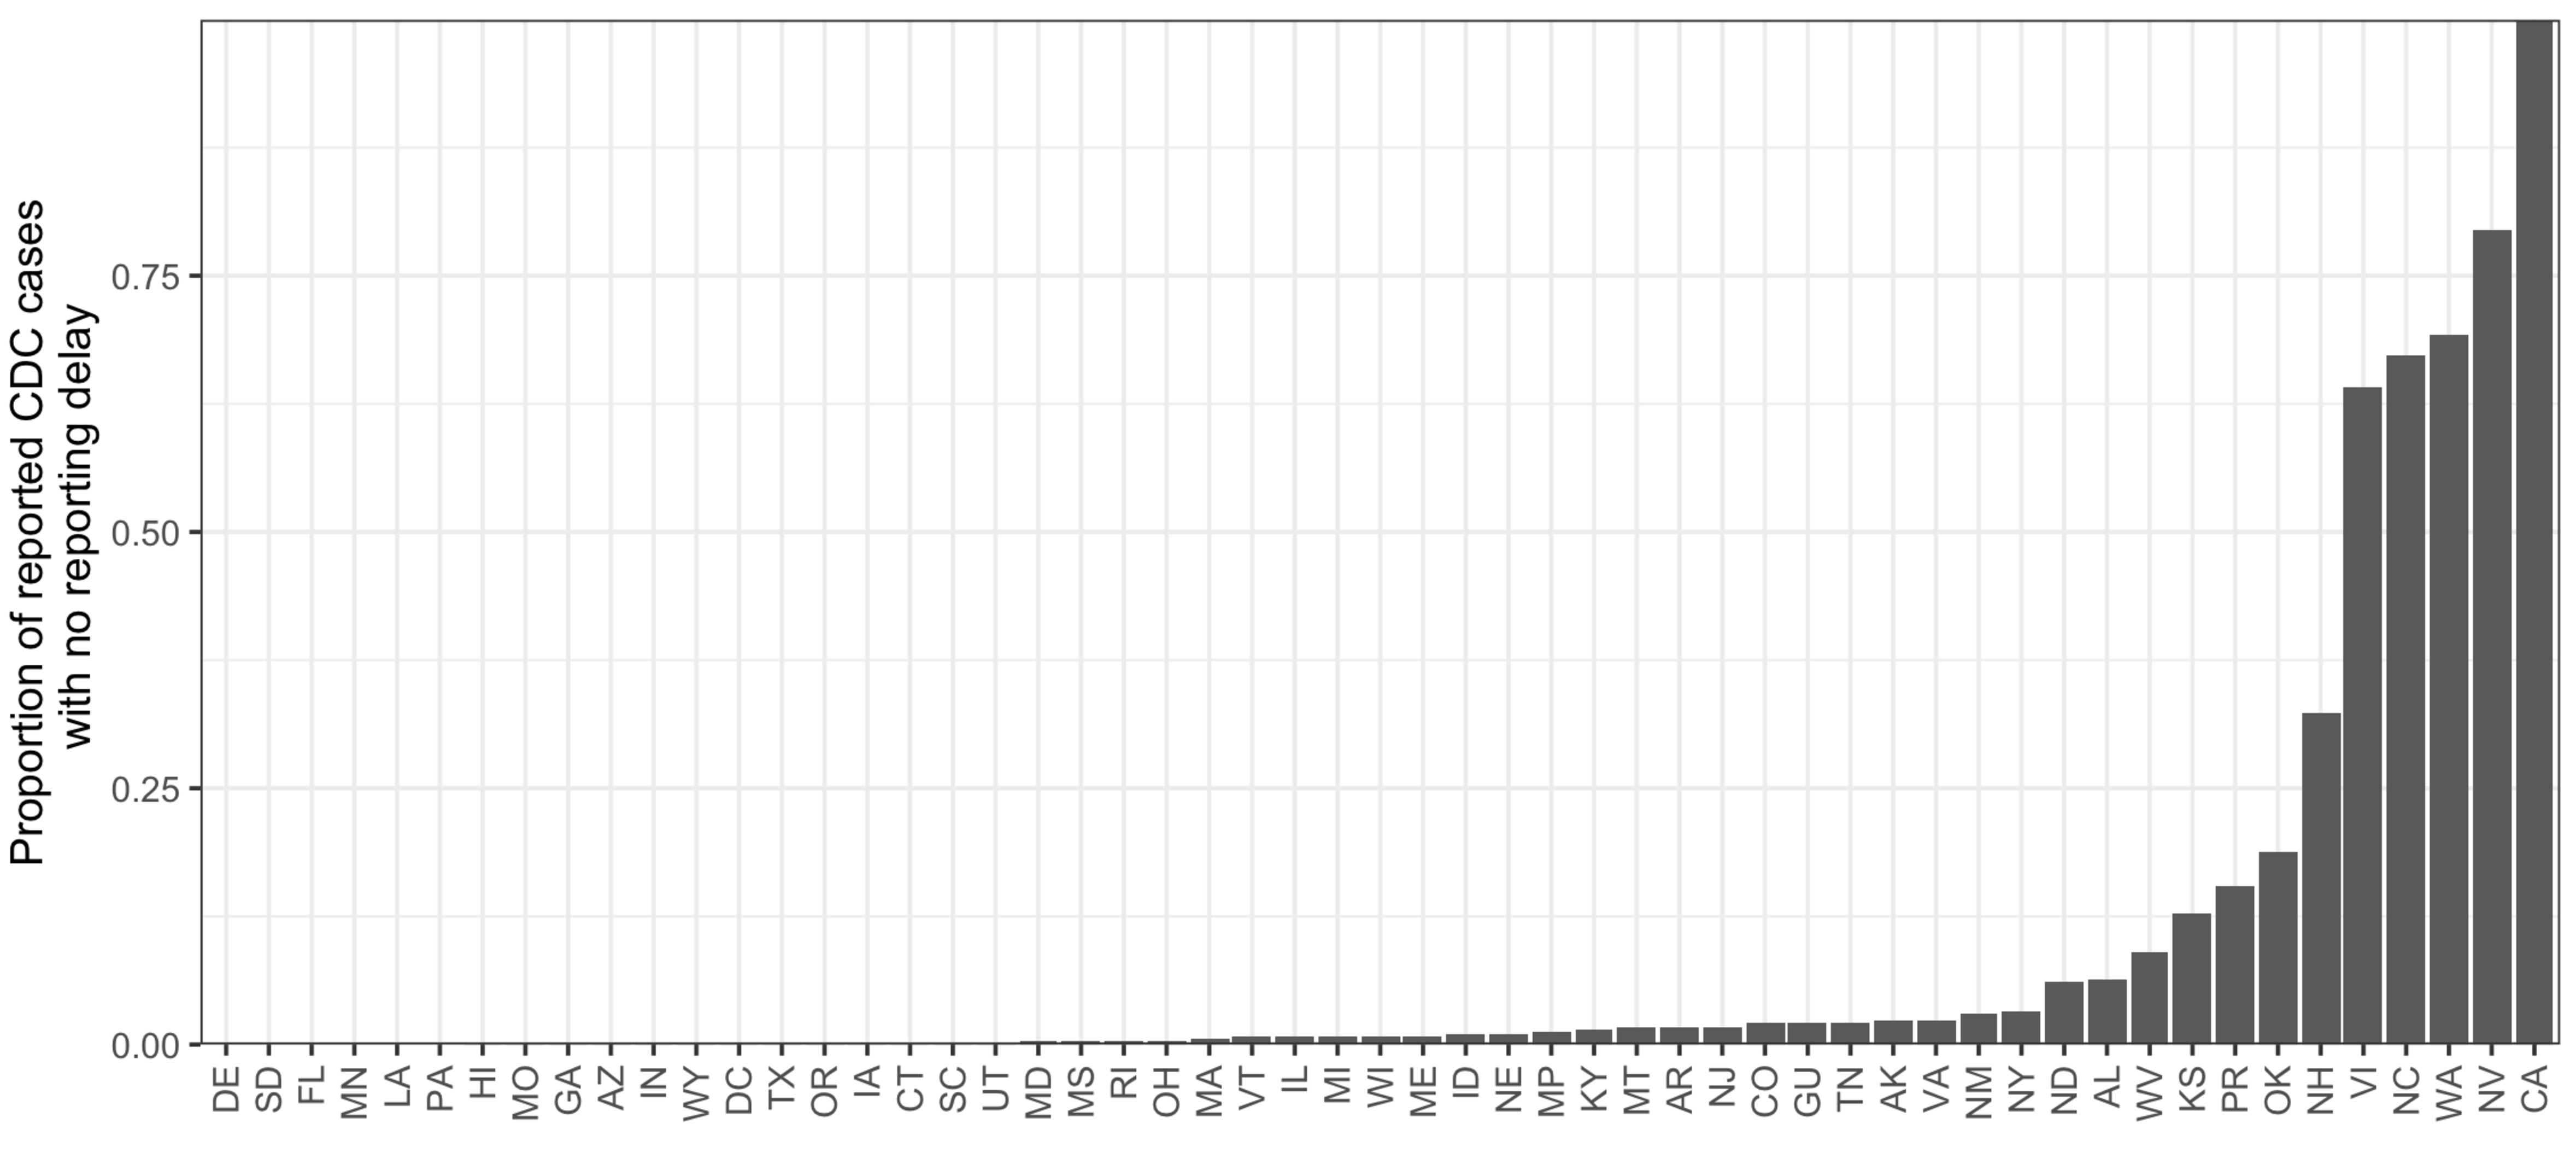
\includegraphics[width=0.9\linewidth]{prop_cc_zero_delay.pdf}\\
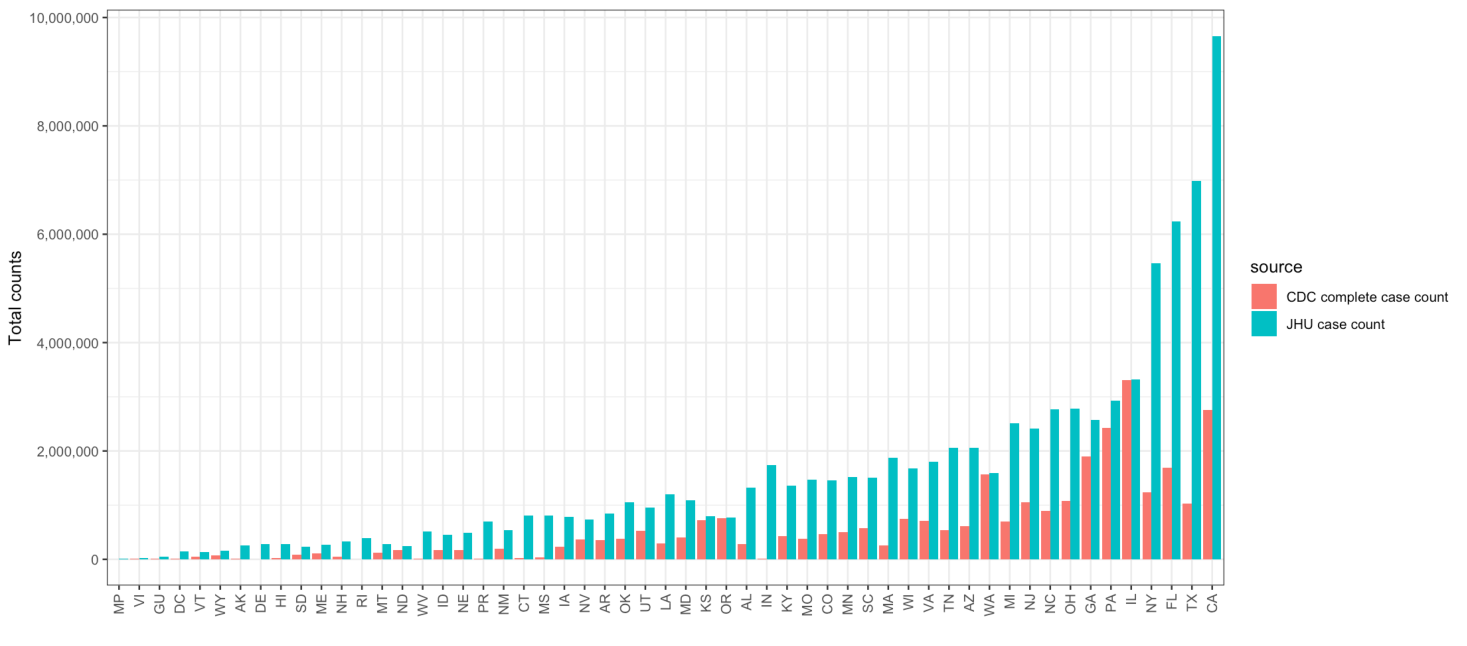
\includegraphics[width=0.9\linewidth]{prop_cc_cdc_vs_jhu.pdf} 
\caption{Top panel: Proportion of complete cases with zero delay between
    positive specimen and report date in the restricted CDC line list dataset.
    Bottom panel: Complete case counts by state in the CDC line list versus the
    cumulative complete case counts from JHU CSSE as of June 6, 2022. All
    counts have been scaled by the 2022 state populations as of July 1, 2022
    from \citep{uscensus2022annual}.}
\label{fig:prop-cc}
\end{figure}

The CDC restricted line list contains 74,849,225 cases (rows) in total compared
to 84,714,805 cases reported by the JHU CSSE; that is, line list is missing
about 10 million cases. The extent that this issue impacts each state is shown
in \Cref{fig:prop-cc}, from which it is clear the fraction of missing cases is
substantial for many states, often surpassing 50\% \citep{jahja2022real}. In
addition, the probability of being missing does not appear to be the same for
states, so there is likely bias introduced from using the complete case line
list data. We consider such bias to be unavoidable in our analysis due to a lack
of alternative line list sources. 



%\subsection{Table on the percent pairwise occurrence of events in the CDC line list}


\subsection{Additional details on delay distribution calculations}
\label{supp:delay-justifications}

In the line list, we observe unusual spikes in reporting in 2020 in comparison
to majority of 2021. When stratified by report date, a few states contribute
unusually large case counts on isolated dates very late in the reporting process
(well beyond 100 days following specimen collection). These large accumulations
of cases over time are likely due breakdowns of the reporting pipeline. Such
anomalies are not likely to be reliable indicators of the delay from positive
specimen to case report. Therefore, we prune these reporting backlogs
systematically. The heuristic is to find large batches of cases that were all
simultaneously reported on the same date with a lengthy delay (as would happen
if a state "found" a tranche of previously unreported positive tests).

For this, we operate only on part of the line list intended for the positive
specimen to case report delay estimation (as this is where we use case reports
from the line list). Then, we divide this line list into three roughly
evenly-spaced and non-overlapping intervals over 2020 and early 2021 (the
interval end points on July 16, 2020, October 16, 2020, and January 15, 2021).
For each interval, we separate the cases with reporting delays that are at least
50 days long into equally-sized bins of 50 days. Then, for each interval and
bin, we perform the following pruning procedure:
\begin{enumerate}[noitemsep]
\item Obtain the total count of these delays for each state. 
\item Check whether each such count on the log scale is at
least the median (for the bin) plus 1.5 times the interquartile range. Retain
only those that exceed this criterion as candidates for pruning. 
\item For the candidate states, compute the case counts by report date. 
\item If there is a report date for a candidate state with a case count greater 
than or equal to a pre-specified threshold, then remove/prune those cases from the line list. 
We set the threshold to be 2000 cases for the first two bins, and then lower
it to 500 for the remaining bins based on inspection.
\end{enumerate}

Finally, in New Hampshire, for a small handful of report dates, all cases
reported by JHU appear in the CDC line list, and all are recorded as having
positive specimen collection date equal to the report date. The resulting
estimate of the delay distribution (see \Cref{sec:step1})
$\widetilde{p}_{\textrm{NH},t}(k)$ would be a point mass at $k=0$ and the weight
$\alpha_{\textrm{NH},t}=1$ resulting $\widehat\pi_{\textrm{NH},t}(k)$ also being a
point mass at $k=0$. In this specific case, we force $\alpha_{\textrm{NH},t} =
\min_{\ell\neq\textrm{NH}} \alpha_{\ell,t}$.

\subsection{Variant circulation proportions}
\label{sec:variant-proportions}


To estimate the daily proportions of the variants circulating in each state, we
obtain the GISAID genomic sequencing data from CoVariants.org
\citep{hodcroft2021covariants, elbe2017data}. These counts represent the total
number of cases belonging to a particular variant using
a sample of positive tests over a biweekly period. To estimate the population
proportion of each variant, we apply multinomial logistic regression 
for the eight variant categories separately for each state. 
Multinomial logistic regression is a standard technique to model the
frequency of SARS-CoV-2 variants 
\citep{obermeyer2022analysis, annavajhala2021emergence, figgins2021sars}.

We let $V_{j\ell,t}$ to be the probability of a new cases at time $t$ in location
$\ell$ corresponding to variant $j$. Let $v_{j\ell,t}$ be the analogous observed
proportion. Then nonparametric multinomial logistic regression models the log odds
as the system
\begin{equation}
\log\left(\frac{V_{j\ell,t}}{1-V_{j\ell,t}}\right) = \beta_{j\ell,0} + \beta_{j\ell,1} t + \beta_{j\ell,2}t^2 + \beta_{j\ell,3}t^3,\;\; j=1,\ldots J.
\end{equation}
This is estimated along with a constraint to ensure that the estimated proportions will sum to 1 across all
$J$ variants. The specification of the log odds as a third-order polynomial in
time produces smoothness of the estimated proportions.
 \Cref{fig:prop_figs} shows the proportions by variant for California before
(left) and after (right) the smoothing procedure. 

\begin{figure}[!tb]
    \centering
        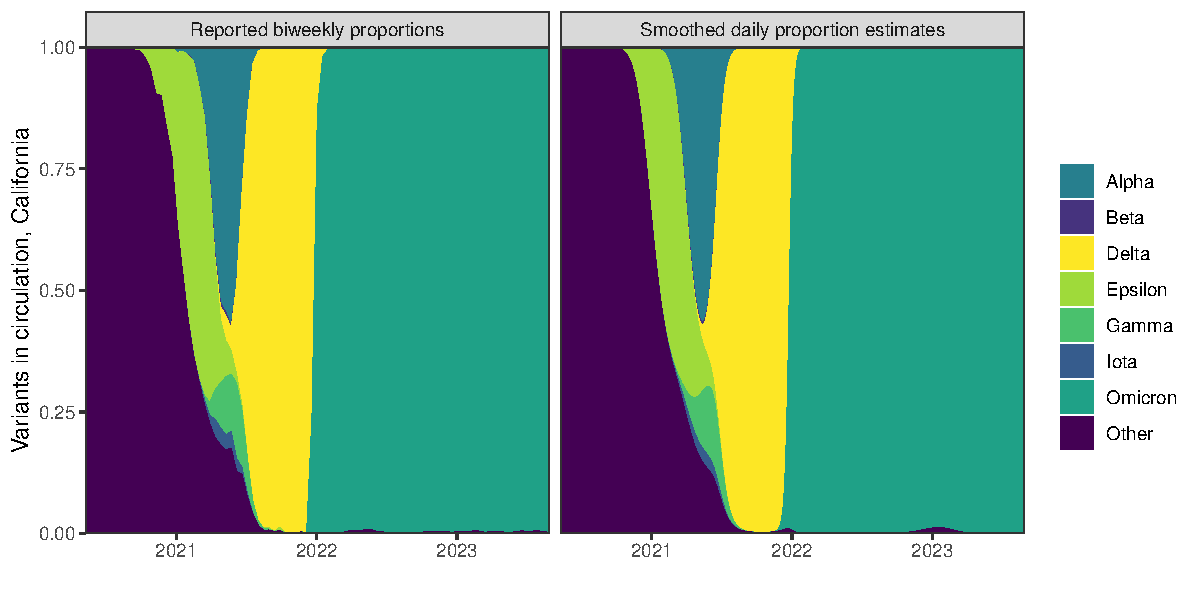
\includegraphics[width=\linewidth]{var-props-1.pdf}
        \caption{Left: Original biweekly proportions of the variants in circulation
        for California. Right: Daily proportions of the variants in circulation for
        California.}
        \label{fig:prop_figs}
    \end{figure}


    


\subsection{Constructing the delay from infection to test}
\label{supp:delay-sops}

The result of Step 1 (\Cref{sec:step1}) is $\widehat{x}_{\ell,t}$, case
estimates by positive specimen date for each state. To continue, pushing this
back to infection estimates, we need the variant-specific delays from infection
to positive specimen collection. As shown in \Cref{fig:chain_events_onset_report}, this delay can be broken into two separate pieces: (1) the
delay from infection to symptom onset, and (2) the delay from symptom onset to
positive specimen collection. The first requires different methods and is
specific to the variant causing the infection, while the second is estimable from the CDC line
list.

\subsubsection{Estimating the incubation period distributions} 
\label{sec:incubation}

To account for the incubation period, the time between infection and symptom
onset, we use estimates from the existing literature, modified slightly for
coherence with each other: we model each incubation as a gamma distribution with
different parameters. We focus on the following eight variants (shown in
\Cref{fig:prop_figs}), which saw significant circulation in one of the \US states
during our study period: Ancestral/Other, Alpha, Beta, Epsilon,
Iota, Gamma, Delta, and Omicron. Alpha, Beta, Delta, Gamma, and Omicron are all
variants of concern \citep{who2021tracking}, while we include the Epsilon
(California) and Iota (New York) variants because of large impact on those and
neighbouring states \citep{yang2022investigation, duerr2021dominance}.

The incubation period of the Ancestral variant has been modelled as a gamma
distribution \citep{tindale2020evidence}, so we simply use the reported shape
and scale parameters. For the Alpha, Beta, Gamma, Delta and Omicron variants,
the mean and standard deviation are reported \citep{tanaka2022shorter,
grant2022impact, ogata2022shorter}. Therefore, we use method of moments to match
the mean and variance to estimate the gamma parameters, using the moment
equations given in \Cref{sec:step1}. Then, we discretize each resulting density
shown in \Cref{fig:inc_gammas} to the support set, which is taken to be from 1
and 21 days. This range assumes that symptoms require at least 1 day to develop
\citealp{phcan2021covid} and that an asymptomatic infection will resolve within
21 days \citep{zaki2021estimations,cortes2022sars}.

We were unable to locate incubation period estimates for the geo-specific
Epsilon and Iota variants, so we use the incubation period for Beta because
Epsilon, Iota, and Beta are all children from the same parent in the
phylogenetic tree of the Nextstrain Clades \citep{hodcroft2021covariants}. All
other circulating variants are grouped together with the Ancestral variant.
There was little available sequencing data prior to Alpha-emergence, but
unfortunately, later in the pandemic, it is impossible to separate Ancestral
from other rare variants, though these also saw minimal circulation after
the middle of 2021.

\begin{figure}[!tb]
\centering
    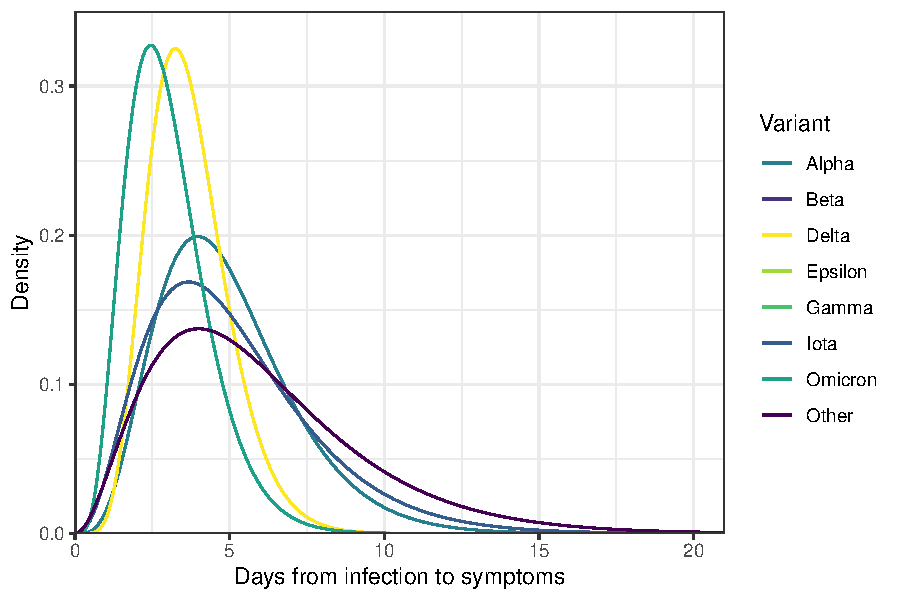
\includegraphics[width=0.6\linewidth]{inc-gammas-1.pdf}
    \caption{Gamma density for the incubation period of each of the eight
    variant categories. Note that the Ancestral variant uses reported shape and
    scale parameters \citep{tindale2020evidence}, while the remaining variants
    convert reported estimates for the mean and variance
    \citep{tanaka2022shorter,grant2022impact,ogata2022shorter} using the method
    of moments to produce the gamma parameters.}
    \label{fig:inc_gammas}
\end{figure}





\subsubsection{Estimating the delay distributions for symptom onset to positive specimen}
\label{supp:delay-sops}


Estimating the delay from symptom onset to positive specimen date follows a
similar procedure as described in \Cref{sec:step1} with a minor
adjustment. Here, we allow $k$ to range from $-3$ to $21$ (rather than $1$ to
$60$). These upper and lower bounds are based on the largest delay values for
the state-wide 0.05 and 0.95 quantiles. The median
delay is very short at approximately 2 days, and an asymptomatic individual may
test positive following a known exposure, before the onset of symptoms. We show
both types of delays for a sample of states over several dates in
\Cref{fig:delay-plots-samp}. Unlike the delay from positive specimen collection
to report, the delay from symptoms to positive specimen can conceivably be
negative. The most obvious reason for this would be if a person knew they had been
exposed to an infectious individual and so got tested prior to the development
of symptoms. Required regular testing for jobs in health care settings,
construction, or the film industry could also produce negative delays.


\begin{figure}[t!]
\centering
    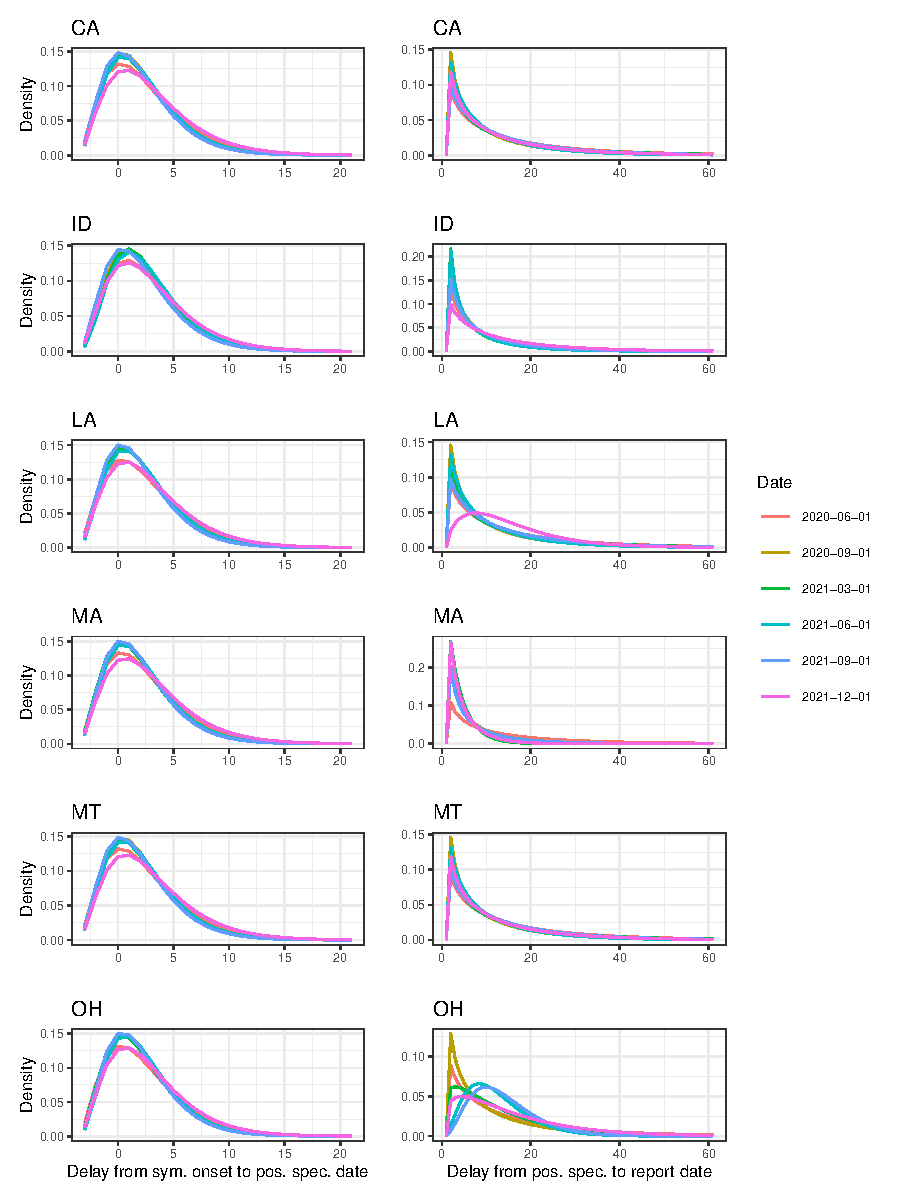
\includegraphics[width=.90\textwidth]{delay_plots.pdf} 
    \caption{Depictions of the estimated delay from symptom onset to
    positive specimen date (left) and from positive specimen date to report date
    (right) for a sample of six states over several dates.}
    \label{fig:delay-plots-samp}
\end{figure}

\subsubsection{Details on constructing the infection-to-test distributions}
\label{supp:details-conv}

Finally, to produce the delay from infection to positive specimen collection we
convolve the variant-specific incubation periods from \Cref{sec:incubation},
denoted by $\{i_{j}(k) : 0 < k \leq 21\}$ with the location-time-specific
symptom-to-positive-test distributions from \Cref{supp:delay-sops}, denoted by
$\{q_{\ell,t}(k) : -3\leq k \leq 21\}$. The convolution of these yields a
distribution $\{\tau_{j\ell,t}(k): -3 \leq k
\leq 42\}$. \Cref{fig:delay-plots-samp} shows the delays used for a sample of 6
states: symptom to positive specimen (left column) and positive specimen to report
(right column). The convolution distribution $\tau_{j\ell,t}$ requires
convolving the distribution in the left column with the variant-specific
incubation periods shown in \Cref{fig:inc_gammas}.





\subsection{Details about seroprevalence data}
\label{supp:sero-details}

We use two major contemporaneous surveys to estimate the proportion of the
population with evidence of previous infection in each state over time: the
2020--2021 Blood Donor Seroprevalence Survey and the Nationwide Commercial Lab
Seroprevalence Survey \citep{cdc2021blood, cdc2021comm}. In the former, the CDC
collaborated with 17 blood collection organizations in the largest nationwide
COVID-19 seroprevalence survey to date \citep{cdc2021blood}. The blood donation
samples were used to construct monthly seroprevalence estimates for nearly all
states from July 2020 to December 2021 \citep{jones2021estimated}. In the latter
survey, the CDC collaborated with two private commercial laboratories to test
blood samples from people that were in for routine or clinical management
(presumably unrelated to COVID-19 \citealp{bajema2021estimated}) for the
antibodies to the virus. The resulting dataset contains seroprevalence estimates
for a number of multi-week collection periods starting in July 2020 to February
2022. 

Both datasets are based on repeated, cross-sectional studies that estimate the
percentage of people who were previously infected with COVID-19 using the
percentage of people from a convenience sample who had antibodies against the
virus \citep{bajema2021estimated, cdc2020data, jones2021estimated}. Adjustments
were made in both for age and sex to account for the demographic differences
between the sampled and the target populations. However, both datasets are
incomplete and they differ in the number and the timing of the data points for
each state (\Cref{fig:sero-blood-comm-compar}). For example, in the
commercial dataset, the last estimate for North Dakota is in September 2020. In
the blood donor dataset, Arkansas does not have estimates available until
October 2020. 

\begin{figure}[!tb]
\centering
    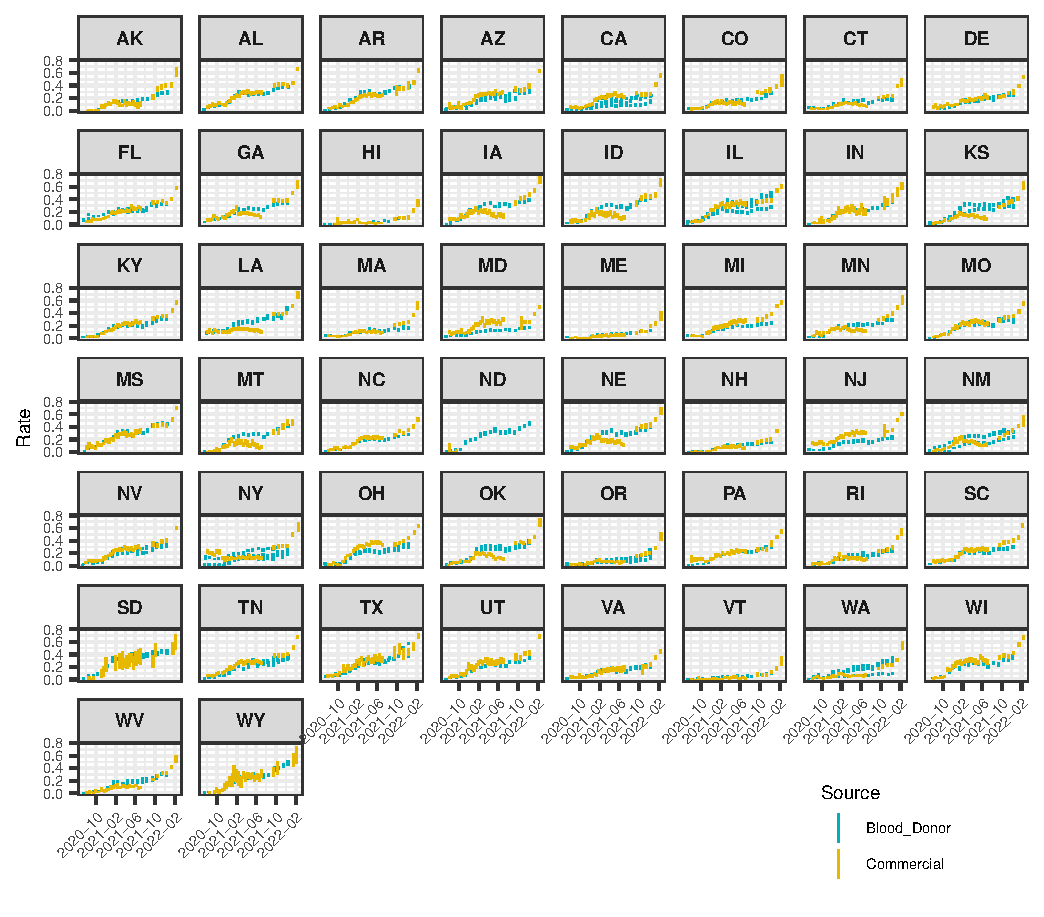
\includegraphics[width=.99\textwidth]{sero_blood_comm_compar.pdf}
    \caption{A comparison of the seroprevalence estimates from the Commercial
    Lab Seroprevalence Survey dataset (yellow) and the 2020--2021 Blood Donor 
    Seroprevalence Survey dataset (blue). Note that the maximum and the minimum
    of the line ranges are the provided 95\% confidence interval bounds to 
    give a rough indication of uncertainty.}
    \label{fig:sero-blood-comm-compar}
\end{figure}
    
A major difference in the structure of the two datasets is that the commercial
dataset always has the seroprevalence estimates at the level of the state, while
the blood donor dataset can either have estimates for the state or for multiple
separate regions within the state. For the commercial dataset, we use the
midpoint of the provided specimen collection date variable.  For the blood donor
dataset, we use the median donation date if the seroprevalence estimates are
designated to be for entire state. If they are instead for regions in the state,
since there is reliably one measurement per region per month, we aggregate the
measurements into one per month per state by using a weighted average (to
account for the given sample sizes of the regions). The median of the median
dates is taken to be the date for the weighted average. If there are multiple
measurements in a week from a seroprevalence source, then the average is used.


\subsection{State space representation of the antibody prevalence
model}\label{supp:ssapm} 

The antibody prevalence model described in \Cref{sec:report-ratio} can be expressed
as a linear Gaussian state space model \citep{durbin2012time}.
For $m = 1, \dots, M$, let $\alpha_m$ be a vector of
latent state processes at time $m$ and $y_m$ be a vector of
observations at time $m$. The form of the (general) linear Gaussian state space model is 
\begin{align}
y_m &= Z\alpha_m + \sigma^2_r\epsilon_m, \qquad \epsilon_m \sim N(0, H_m) \label{eq:ss1}\\
\alpha_{m+1} &= T_m\alpha_m + R\eta_m, \quad \eta_m \sim N(0, Q) \label{eq:ss2}
\end{align}
where $\alpha_1 \sim N(a_1, P_1)$ and 
$\epsilon_m$ and $\eta_m$ are mutually and serially independent.

% Kalman filtering gives the following one-step-ahead predictions of the states
% \begin{align*}
% a_{t+1} &= \E[\alpha_{t+1}\given y_t, \dots, y_1] 
% \end{align*} with covariance,
% \begin{align*}
% P_{t+1} &= \Var(\alpha_{t+1} \given y_t, \dots, y_1).
% \end{align*}
% Then, the Kalman smoother works backwards to the first time to give
% \begin{align}
% \hat{a}_t &= \E[\alpha_{t}\given y_n, \dots, y_1] \label{eq:hatat}\\
% V_t &= \Var(\alpha_{t}\given y_n, \dots, y_1). \label{eq:Vt}
% \end{align}
% The filtering and smoothing steps are based on recursions that are described in
% Appendix A of \citep{helske2017kfas} as we use the R package KFAS to estimate
% our model.

% For our situation, the Kalman filter and smoothing approach offers a number of
% advantages over the penalized regression approach. Perhaps most notably,
% the parameters are estimated all at once (so cross validating for model
% parameter tuning is not necessary). Another major benefit is that it can handle 
% unevenly spaced time series (refer to \citealp{durbin2012time} for further details).

To express the antibody prevalence model in state space form, we relate the
model in \Crefrange{eq:sero-measurements}{eq:report-ratio} to the components in
\Cref{eq:ss1,eq:ss2} as follows (omitting the location subscript for
simplicity):

% Probably move the below specification to the appendix

\begin{align*}
    Z &= \begin{bmatrix} 1 & 0 & 0 & 0 \\ 0 & 1 & 0 & 0 \end{bmatrix} &
    H_m &= \begin{bmatrix}w^1_{m} & 0 \\ 0 & w^2_{m} \end{bmatrix} \\
    \alpha_m &= \begin{bmatrix}s_{m} \\ a_m \\ a_{m-1}\\ a_{m-2} \end{bmatrix} & 
    T_m &= \begin{bmatrix}(1 - \gamma) & \widehat{u}^\Sigma_{m} (1 - z_m) & 0 & 0\\ 
        0 & 3 & -3 & 1 \\ 0 & 1 & 0 & 0\\ 0 & 0 & 1 & 0 \end{bmatrix}  & 
    R &= \begin{bmatrix}1 & 0  \\ 0 & 1 \\ 0 & 0 \\ 0 & 0 \end{bmatrix}\\
    Q &= \begin{bmatrix} \sigma^2_\epsilon & 0  \\ 0 & \sigma^2_\eta \end{bmatrix} &
    a_1 &= \begin{bmatrix} \tilde{s}_{1}\\ \tilde{a}_1\\ \tilde{a}_1 \\ \tilde{a}_1 \end{bmatrix} & 
    P_{1} &= \begin{bmatrix} \sigma^2_{\tilde{s}_{1}} & 0 & 0 & 0 \\ 
    0 & \sigma^2_{\tilde{a}_1} & 0 & 0\\ 0 & 0 & \sigma^2_{\tilde{a}_1} & 0 \\ 
    0 & 0 & 0 & \sigma^2_{\tilde{a}_1} \end{bmatrix} 
\end{align*}
where $\sigma^2_r$ is the variance of observations, $\sigma^2_\epsilon$ is the
variance of the seroprevalence estimates, $\sigma^2_\eta$ is the trend variance,
and $\widehat{u}^\Sigma_{m}$ denotes the new deconvolved cases between $m$ and
$m+1$. Because the inverse reporting ratios should be more variable than the
seroprevalence estimates, we enforce that the estimate of $\sigma^2_\eta$ is a
multiple of $\sigma^2_\epsilon$. 

Finally, $w^1_{m}$ and $w^2_{m}$ are the time-varying inverse variance weights
computed from the commercial and blood donor datasets, respectively. For each
source, we compute the weights for the observed seroprevalence estimates using
the formula for the standard error of a proportion. These weights are then
re-scaled to sum to the number of observed seroprevalence measurements for the
source. Finally, the ratio of the average observed weights from the two sources
is used to scale all weights relative the commercial source. This transformation
is done purely for computational purposes to make estimation of the unknown
parameters easier.

The prior distribution for $\alpha_1$ is estimated using both data-driven
constraints and externally sourced information. The initial value of the
seroprevalence component, $\tilde{s}_{1}$ is the average of the initial
seroprevalence measurements from each source rounded down to two decimal places,
The corresponding initial variance estimate, $\sigma^2_{\tilde{s}_{1}}$, is
taken to be the mean of the standard errors of the two seroprevalence estimates.
For the initial values of the trend components, we use the inverse of the
ascertainment ratio estimate for each as of June 1, 2020 from Table 1 in
\citep{unwin2020state}: the mean for $\tilde{a}_1$ and half the width of the
confidence interval converted to the inverse for
$\sigma^2_{\tilde{a}_1}$.

The initial $\sigma^2_r$ is taken to be the average of the estimated variances
from the observed seroprevalence measurements regressed linearly on time.
The initial value of the multiplier is set to be $100$ for all states. The
$\sigma^2_\epsilon$ and $\gamma$ values are estimated separately for each state,
then fixed to their averages on the log-scale.

Following maximum likelihood estimation of remaining parameters we use the
Kalman filter to obtain the smoothed point estimates and variances of the weekly
inverse reporting ratios. We use forward and backward extrapolation to extend
these estimates outside of the observed seroprevalence range
\citep{durbin2012time}, followed by linear interpolation to produce daily
values. We then multiply these by the
corresponding deconvolved case estimates before converting to per-capita values.
Annual estimates of the state
populations as of July 1 of 2020 are taken from the Dec.\
2022 press release from the \US Census Bureau \citep{uscensus2022annual}.


% The $50$, $80$, and $95\%$ confidence intervals are constructed by taking a
% Bayesian view of the antibody prevalence model (refer to \ref{supp:bayeswaning} 
% for the Bayesian specification of the model). 
% That is, for each time, $t$, we obtain an estimate of the
% posterior variance of $a_t$, apply the deconvolved case estimate as a constant
% multiplier, and then use resulting variance to build a normal confidence
% interval about the infection estimate. We additionally enforce that the lower
% bound must be at least the deconvolved case estimate for the time under consideration.


% \subsection{Bayesian specification of the antibody prevalence
% model}\label{supp:bayeswaning} 
% In brief, the antibody prevalence model where we let
% $\beta = \left \{  \gamma, a_1,\dots, a_t \right \}$ and $X$ be the design
% matrix, corresponds to a Bayesian model with prior 
% \begin{align*}
%     \beta \sim N \left( 0,  \frac{\sigma^2 }{ \lambda} \left( A^TD^TDA 
%     \right)^{-1}  \right)
% \end{align*} and likelihood 
% \begin{align*}
%     s|X,\beta \sim N \left( X\beta, \sigma^2W^{-1} \right),
% \end{align*} where $A$ is indicator matrix save for the first column of $0$s 
% (corresponding to $\gamma$), $D$ represents the discrete derivative matrix of 
% order $3$, and $W$ is the inverse variance weights matrix. Then, the posterior 
% on $a_t$ is normally distributed with mean 
% \begin{align*}
%     \left ( X^TWX + \lambda A^TD^TDA \right )^{-1}X^TWs
% \end{align*} 
% and variance 
% \begin{align*}
%     \sigma^2 (X^TWX + \lambda A^TD^TDA)^{-1}.
% \end{align*}


% \subsection{Scaling by population}



% \subsection{Ablation analysis of infection-hospitalization correlations}

% To better understand the contribution of the intermediate steps to the lagged
% correlation analysis, we carry out a brief ablation study in which we calculate
% the lagged correlation using the following infection estimates: 1. those from
% the deconvolution procedure under the assumption that the infection onset is the
% same as the positive specimen date (i.e., excluding the positive specimen to
% infection onset data and deconvolution); 2. those from the deconvolution
% procedure under the assumption that the infection onset is the same as the
% symptom onset date (excluding the incubation period data); 3. those from the
% deconvolution procedure when utilizing all incubation period and delay data (the
% deconvolved case estimates); 4. those from applying the antibody prevalence
% model to produce estimates for both the reported and the unreported cases (the
% infection estimates).

% The results of this study are shown in \Cref{fig:abl-lag-cor}. From
% this, we can see that the deconvolved case and infection estimates from the
% intermediate steps are all leading indicators of hospitalizations. However, the
% degree that each such set of estimates lead hospitalizations depend on its
% location in the sequence of deconvolution steps and how close the estimates are to infection
% onset. For example, the deconvolved cases by positive specimen date tend to
% precede hospitalizations by about $11$ days, while those for the subsequent step
% indicate that the deconvolved cases by symptom onset tend to precede
% hospitalizations by a longer time of $13$ days. Finally, after adding the
% variant-specific incubation period data into the deconvolution and obtaining the
% deconvolved case estimates, we can observe that the reported infections precede
% hospitalizations by about $19$ days. 

% \begin{figure}[H]
% \centering
%     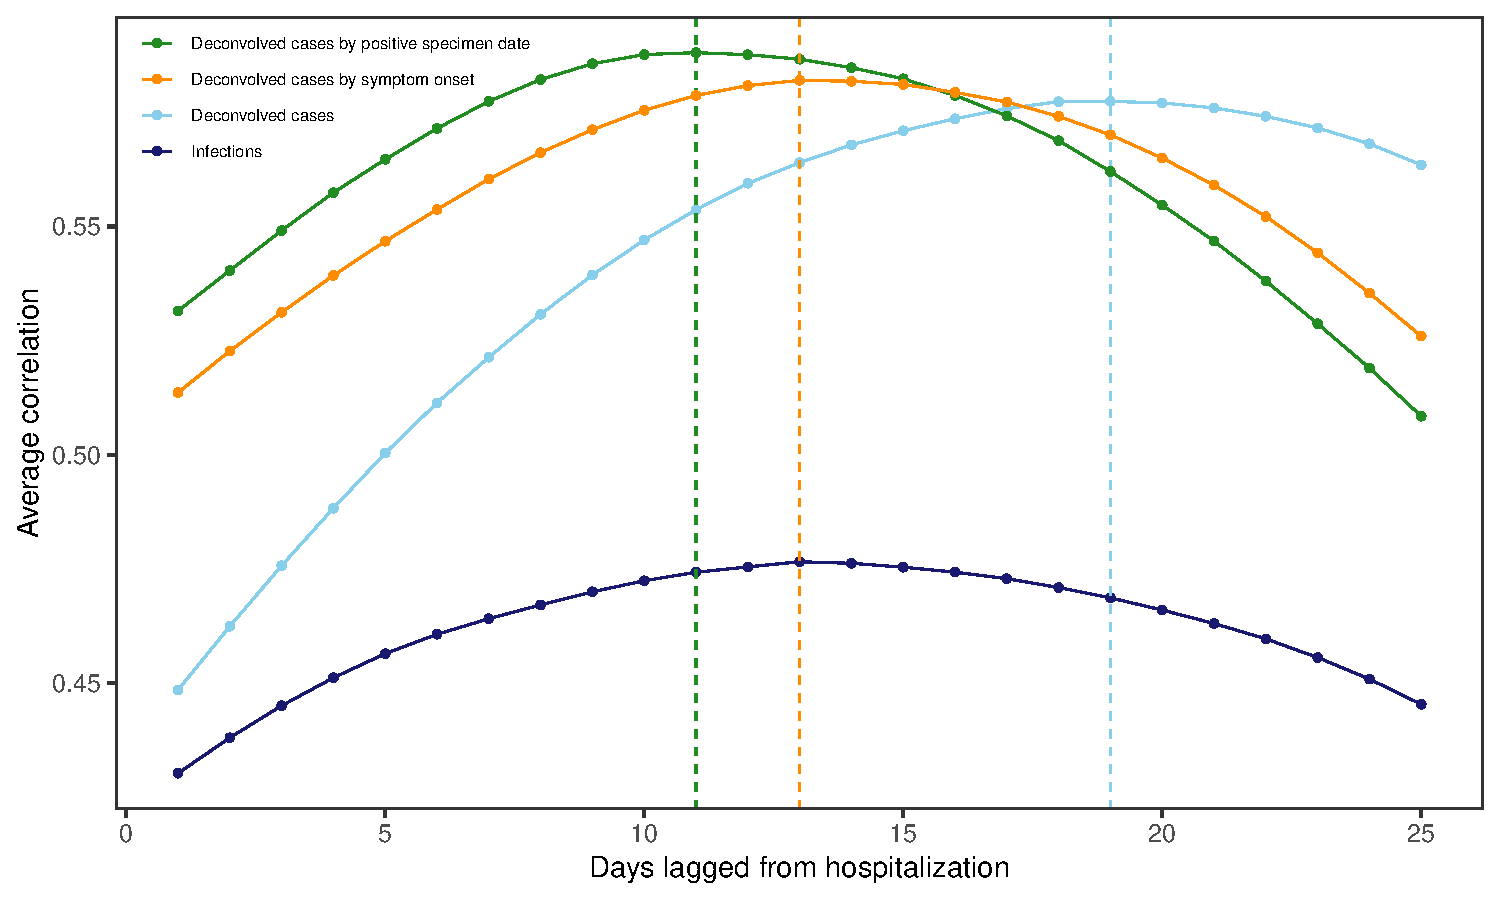
\includegraphics[width=.78\textwidth]{adj_unadj_pi_no_inc_hosp_lag_corr_F24.pdf} 
%     \caption{Lagged Spearman's correlation between the infection and
%     hospitalization rates per 100,000 averaged for each lag across \US states
%     and days over June 1, 2020 to November 29, 2021, and taken over a rolling
%     window of 61 days. The infection rates are based on the counts for the
%     deconvolved case and infection estimates as well as the reported infections
%     by symptom onset and when the report is symptom onset. Note that each such
%     set of infection counts is subject to a center-aligned 7-day averaging to
%     remove spurious day of the week effects. The dashed lines indicate the lags
%     for which the highest average correlation is attained.}
%     \label{fig:abl-lag-cor}
% \end{figure}
 

\end{document}